\input{../header}
\usepackage{pgfplots}
\rhead{Your name: \rule{8cm}{0.15mm}}

\begin{document}
%
\section{Learning target DF0, version 1}
Compute and interpret average velocity and its units, using information about the position function (as a table, graph, and/or function formula).

\hrulefill

The position (in miles), $s(t)$, of a car driving along a straight road at time $t$ (in minutes), is given by the following graph. \\
		
	%	\begin{center}
		\scalebox{0.35}{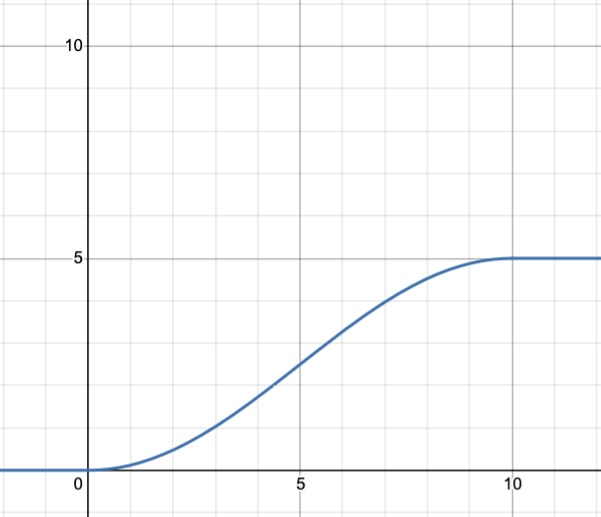
\includegraphics{../images/LT1-1-S24.jpg}}
	%	\end{center}
		
\begin{enumerate}
	\item Determine the average velocity of the car between $t=5$ and $t=10$ minutes, $AV_{[5,10]}$. Use proper notation and the work you did to determine the result; include units on your answer.

	\vspace{1in}

	\item On the graph of $s(t)$ draw a line through  $(3,s(3))$ and $(7,s(7))$; what is the slope of this line and what does that slope mean in the physical context of the function $s$?  
	
	\vspace{0.85in}
	
	
	\item Here's some additional data for the function $s(t)$ that's pictured above: 
	
	\begin{center}
		\begin{tabular}{|c|c|c|c|c|}
			\hline
			$t$ (in minutes) & 8.0 & 8.05 & 8.1 & 8.15 \\
			\hline
			$s(t)$ (in miles) & 4.52254 & 4.54537 & 4.56770 & 4.58952\\
			\hline
		\end{tabular}
	\end{center} 
	
	Find the average velocity of the car on the interval $[8.05, 8.1]$. Label your result using proper notation and include units on your answer.
	
\end{enumerate}
%%%%%%%%%%%%%%%%%%%%%%%%%%%%%%%%%%%%%%%%%%%%%%%%%%%%%%%%%
\pagebreak
%%%%%%%%%%%%%%%%%%%%%%%%%%%%%%%%%%%%%%%%%%%%%%%%%%%%%%%%%

\section{Learning target DF0, version 2}
Compute and interpret average velocity and its units, using information about the position function (as a table, graph, and/or function formula).

\hrulefill
\begin{enumerate}[leftmargin=10pt]

	\item Your fitbit records some data about the distance you traveled on a bike ride around the city:
	
	\begin{center}
		\begin{tabular}{|c|c|c|c|c|c|c|}
		\hline
		$t$ (in minutes) & 0 & 15 & 30 & 45 & 60 & 75 \\
		\hline
		$d(t)$ (in miles) & 0 & 4.5 & 10.5 & 15 & 21 & 24\\
		\hline
		\end{tabular}
		\end{center}
	Find your average velocity over the time interval from $t = 30$ to $t = 75$. Include units.
	
	\vfill

	\item The following graph shows a plot of the function $s(t)$ that measures the location of a car (in thousands of feet) along a road at time $t$ in minutes.
	
	\begin{center}
	\scalebox{0.65}{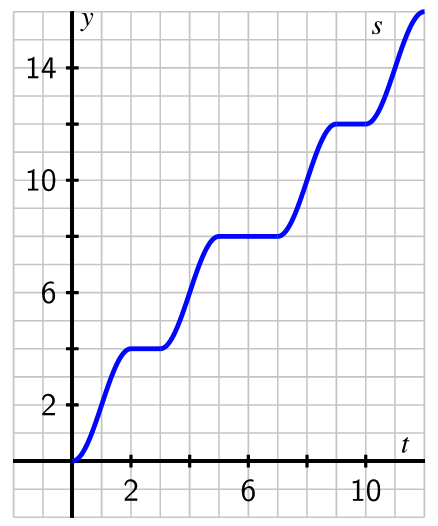
\includegraphics{../images/CP-3-01-s.png}}
	\end{center}
		
	\begin{itemize}
		\item Use the graph to find the average velocity of the car between $t=2$ and $t=7$ minutes, $AV_{[2,7]}$. Include units on your answer.
		
		
		\vfill

		\item On the graph of $s(t)$ draw a line through $(7,s(7))$ and $(10,s(10))$; what is the slope of this line, and what does that slope mean in the physical context of the function $s$?  Include units on your answer.
		
		
	\end{itemize}

\end{enumerate}
%%%%%%%%%%%%%%%%%%%%%%%%%%%%%%%%%%%%%%%%
\pagebreak
%%%%%%%%%%%%%%%%%%%%%%%%%%%%%%%%%%%%%%%%

\section{Learning target DF1, version 1}

Estimate the value of a derivative using difference quotients, and draw corresponding secant and tangent lines on the graph of a function.

\hrulefill


\everymath{\displaystyle}

Suppose that you know the following values of some function $g(x)$:

\[
\begin{array}{c||r|r|r}
      x  &  1.7 &  2   &  2.3 \\\hline
    g(x) & -2.2 & -2   & -1.5
\end{array}
\]
\begin{enumerate}[leftmargin=0pt]

\item Plot these points and sketch a plausible graph of $g(x)$.

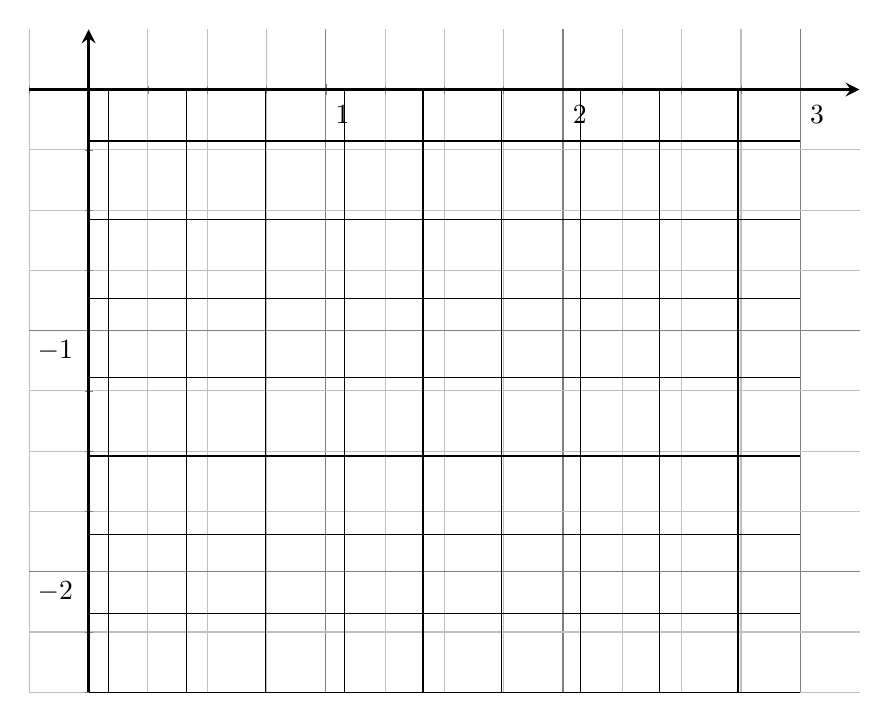
\begin{tikzpicture}
    \begin{axis}[
        width=\textwidth, height=10cm,
        xmin=-0.25, xmax=3.25, ymin=-2.5, ymax=0.25,
        xtick distance = 1, ytick distance = 1,
        minor tick num = 3,
        xticklabel style={anchor=north west},
        yticklabel style={anchor=north east},
        major grid style={thin, black!50},
        grid=both, 
        axis lines=center, axis line style = very thick]
        \draw (0,0) grid (3, -3);
    \end{axis}
\end{tikzpicture}

\item On your graph above, draw a plausible tangent line to the graph of $g(x)$ at $x=2$.

\item Use a central difference to estimate $g'(2)$. Draw the corresponding secant line on your graph above.

\vfill

\item Compute another, different estimate of $g'(2)$. Draw the corresponding secant line on your graph.

\vfill

\item Which one of your approximations is the best? How do you know?

\vspace{1cm}

\end{enumerate}

%%%%%%%%%%%%%%%%%%%%%%%%%%%%%%%%%%%%%%%%%%%%%%%%%%%%%%%%%
\pagebreak
%%%%%%%%%%%%%%%%%%%%%%%%%%%%%%%%%%%%%%%%%%%%%%%%%%%%%%%%%

\section{Learning targets DF1 and DFa, version 2}

Arapaho Glacier is a mountain glacier in Roosevelt National Forest,
west of Boulder, CO. The following table\footnote{
Haugen, B., Scambos, T., Pfeffer, T., \& Anderson, R. (2010). Twentieth-century changes in the thickness and extent of Arapaho Glacier, Front Range, Colorado. \textit{Arctic, Antarctic, and Alpine Research, 42}(2), 198-209.}
gives the surface area, $A(t)$, in square meters, of Arapaho Glacier in the year $t$. 
\begin{center}
	\begin{tabular}{|c|c|c|c|c|}
	\hline
	$t$ & 1900 & 1960 & 1973 & 1999\\
	\hline
	$A(t)$ & 338,282 & 250,764 & 225,000 & 162,027\\
	\hline
	\end{tabular}
 \end{center}
	
\begin{enumerate}[leftmargin=0pt]

\item Compute an approximation for $A'(1960)$, and {\bf include units} for this number.
\vfill
\item Write a sentence explaining what the number means about how the area of the glacier is changing.\\
\textbf{Don't say ``per,'' and don't say ``rate.''}

\vfill
\vfill

\item Compute an approximation for $A'(1999)$, and {\bf include units} for this number.\\
Do you think your approximation is too high or too low? Why?

\vfill
\vfill

\item How does $A'(1960)$ compare to $A'(1999)$? Is that good or bad?
\vfill
\end{enumerate}

%%%%%%%%%%%%%%%%%%%%%%%%%%%%%%%%%%%%%%%%%%%%%%%%%%%%%%%%%
\pagebreak
%%%%%%%%%%%%%%%%%%%%%%%%%%%%%%%%%%%%%%%%%%%%%%%%%%%%%%%%%

\section{Learning target DF1, version 3}


Estimate the value of a derivative using difference quotients, and draw corresponding secant and tangent lines on the graph of a function.

\hrulefill


Below is a graph of the function $\displaystyle f(x)=\frac{x^4}{12}-\frac{x^2}{2}-x$. 
\begin{center}
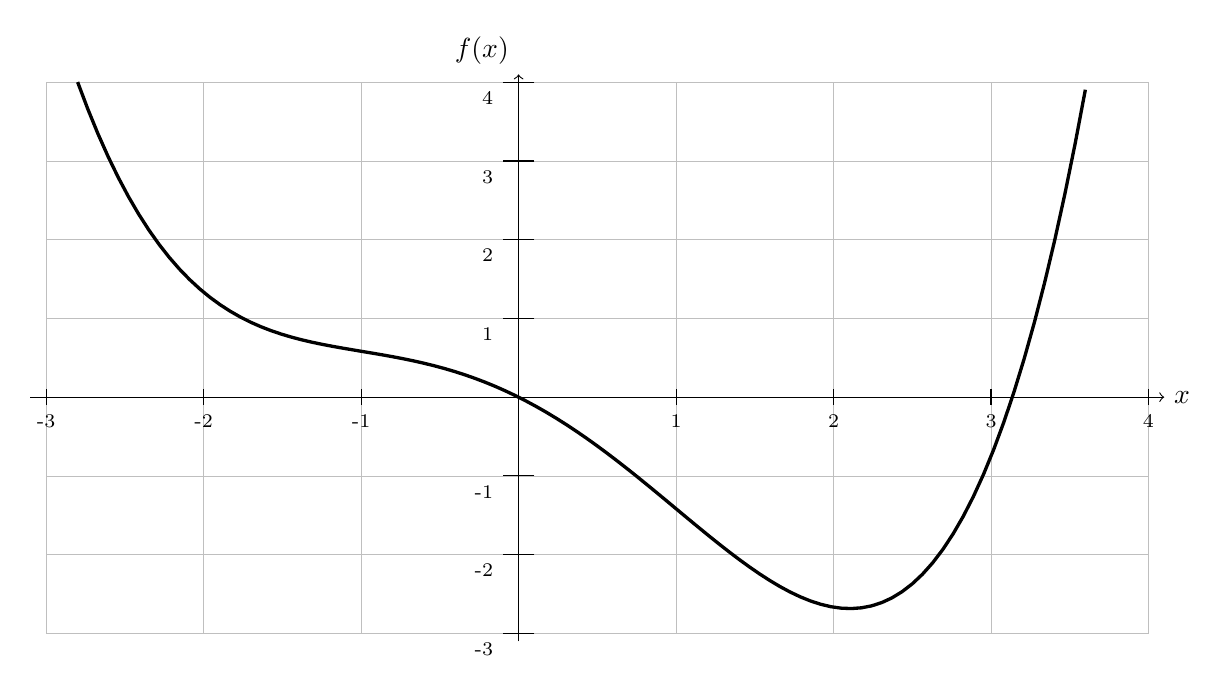
\begin{tikzpicture}[domain=-4:4, xscale = 2, yscale = 1] 
%grid and axis: 
\draw[very thin, color=lightgray] (-3,-3) grid (4,4);
\draw[->] (-3.1, 0) -- (4.1, 0) node[right] {$x$};
\draw[->] (0, -3.1) -- (0, 4.1) node[above left] {$f(x) $};

%x-axis labels:
\foreach \i in {-3,-2,-1,1, 2, 3,4} {
	\draw (\i, .1) -- (\i, -.1) node[below] {\scriptsize \i};
}
%y-axis labels:
\foreach \i in {-3,-2,-1, 1, 2, 3, 4} {
	\draw (.1,\i) -- (-.1, \i) node[below left] {\scriptsize \i};
}
\draw[very thick, color=black, domain=-2.8:3.6, samples=100] plot (\x,{0.08333*\x*\x*\x*\x-0.5*\x*\x-\x}) node[] {};
\end{tikzpicture}
\end{center}

\begin{enumerate}[(a)]
\item On the graph above, draw the tangent line to the curve at $x=-1$. 

\item On the graph above, draw a secant line that goes through the curve at $x=-1$ and at some other nearby $x$-value of your choice.

\item Calculate the slope of that secant line.

\vfill

\item Use $f'(x)$ to calculate the slope of the tangent line. Compare the value you get here to the value you got in part (c). Does that make sense?

\vfill
\end{enumerate}

%%%%%%%%%%%%%%%%%%%%%%%%%%%%%%%%%%%%%%%%%%%%%%%%%%%%%%%%%
\pagebreak
%%%%%%%%%%%%%%%%%%%%%%%%%%%%%%%%%%%%%%%%%%%%%%%%%%%%%%%%%


\section{Learning target DF1, version 4}

Estimate the value of a derivative using difference quotients, and draw corresponding secant and tangent lines on the graph of a function.

\hrulefill

A water balloon is tossed vertically in the air from a window. The balloon's height (measured in feet) at time $t$ (measured in seconds after being launched) is given by \(s(t) = -16t^2 + 16t + 32\); \\
a graph of this function is provided below.

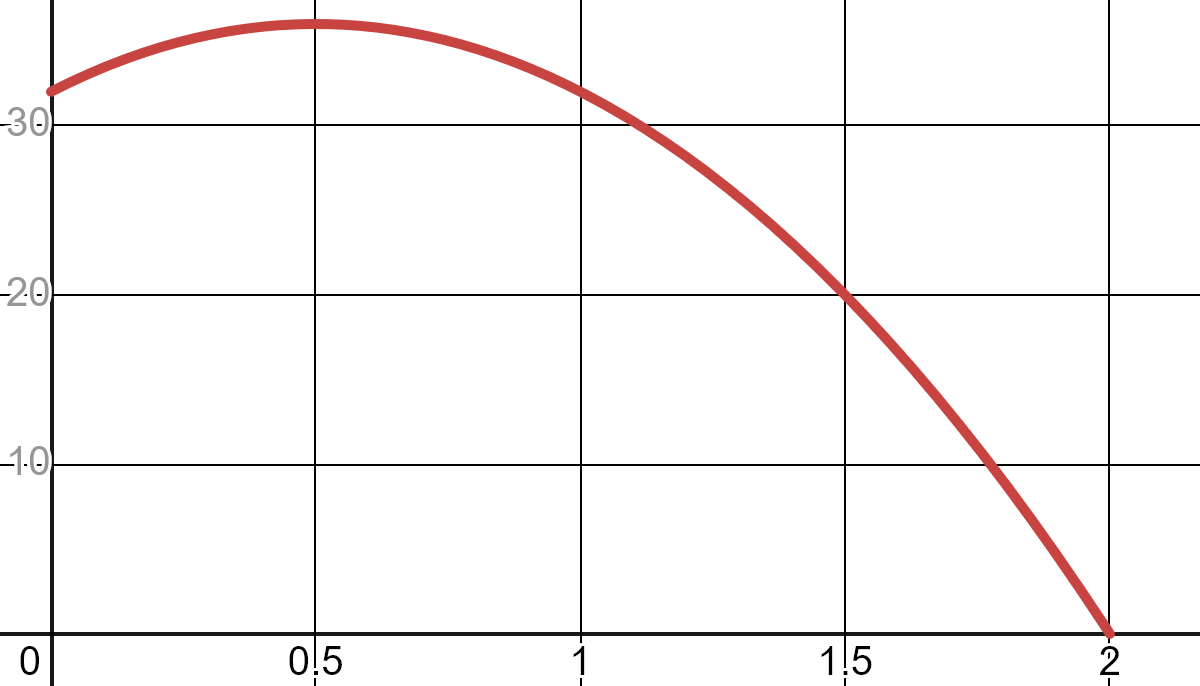
\includegraphics[width=\textwidth]{../images/DF1-v4.png}

\begin{enumerate}[(a)]
    \item Compute $s(1)$. Show your work.
    \vfill
    \item On the graph above, carefully sketch the \textit{tangent} line to $s(t)$ at $t=1$.
    \item On the graph above, carefully sketch a \textit{secant} line through the point on the graph at $t=1$ and a second nearby point.
    \item Compute the slope of your secant line. Show your work and \textbf{include units}. 

    \vspace{-0.7em}
    {\tiny Hints: rise over run; one of your two $y$-values is $s(1)$, which you computed in part (a).}
    \vfill
    \item Use shortcut rules to find $s'(t)$, and compute $s'(1)$; show your work. Compare your result here to your result in part (d). Do these two numbers make sense together? Why?
    \vfill
\end{enumerate}

%%%%%%%%%%%%%%%%%%%%%%%%%%%%%%%%%%%%%%%%%%%%%%%%%%%%%%%%%
\pagebreak
%%%%%%%%%%%%%%%%%%%%%%%%%%%%%%%%%%%%%%%%%%%%%%%%%%%%%%%%%

\section{Learning target DF1, version 5}

Estimate the value of a derivative using difference quotients, and draw corresponding secant and tangent lines on the graph of a function.

\hrulefill


\everymath{\displaystyle}

Suppose that you know the following values of some function $f(x)$:

\[
\begin{array}{c||r|r|r}
      x  &  1 &  1.5   &  2 \\\hline
    f(x) & -0.8 & -1   & -1.6
\end{array}
\]
\begin{enumerate}[leftmargin=0pt]

\item Plot these points and sketch a plausible graph of $f(x)$.

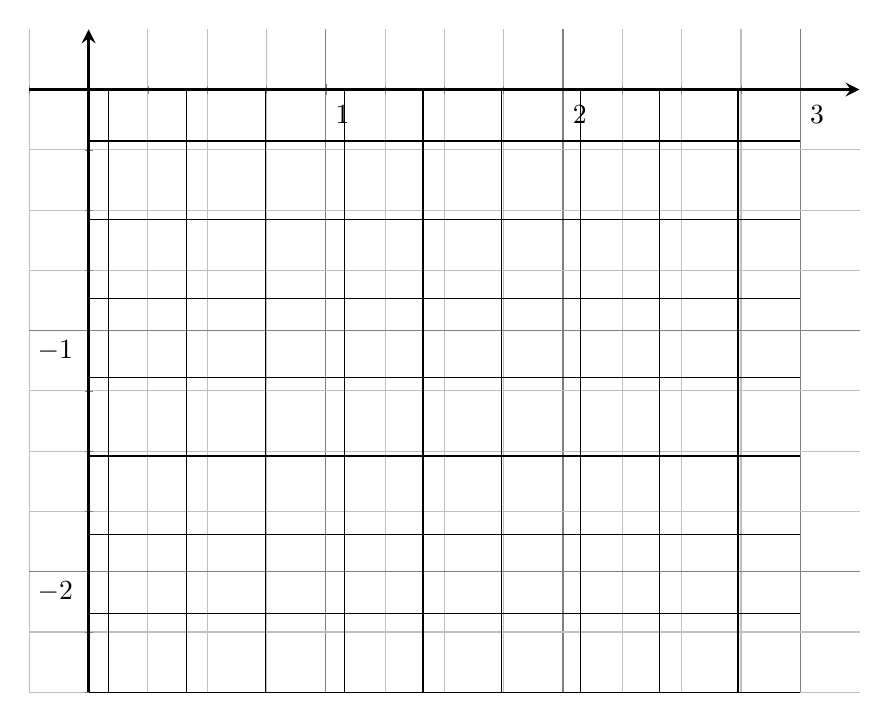
\begin{tikzpicture}
    \begin{axis}[
        width=\textwidth, height=10cm,
        xmin=-0.25, xmax=3.25, ymin=-2.5, ymax=0.25,
        xtick distance = 1, ytick distance = 1,
        minor tick num = 3,
        xticklabel style={anchor=north west},
        yticklabel style={anchor=north east},
        major grid style={thin, black!50},
        grid=both, 
        axis lines=center, axis line style = very thick]
        \draw (0,0) grid (3, -3);
    \end{axis}
\end{tikzpicture}

\item On your graph above, draw a plausible tangent line to the graph of $f(x)$ at $x=1.5$.

\item Use a central difference to estimate $f'(1.5)$. Draw the corresponding secant line on your graph.
\vfill

\item Compute another, different estimate of $f'(1.5)$. Draw the corresponding secant line on your graph.

\vfill

\item Which one of your approximations is the best? How do you know?

\vspace{1cm}

\end{enumerate}
%%%%%%%%%%%%%%%%%%%%%%%%%%%%%%%%%%%%
\pagebreak
%%%%%%%%%%%%%%%%%%%%%%%%%%%%%%%%%%%%


\section{Learning target DF2, version 1}

Find derivatives using the definition of derivative as a limit.

\hrulefill

Suppose that $f(x) = 3x^2 - 5x + 4$. Use the limit definition of the derivative to find $f'(x)$. 

\vfill

PS: The answer is $f'(x) = 6x - 5$.
%%%%%%%%%%%%%%%%%%%%%%%%%%%%%%%%%%%%%%%%%%%%%%%%%%%%%%%%%
\pagebreak
%%%%%%%%%%%%%%%%%%%%%%%%%%%%%%%%%%%%%%%%%%%%%%%%%%%%%%%%%

\section{Learning target DF2, version 2}

Find derivatives using the definition of derivative as a limit.

\hrulefill

Suppose that  \(g(w) = 6 \, w^{3} - 2 \, w^{2} - 9 \, w - 2\). Use the limit definition of the derivative to find $g'(w)$.

\vspace{1em} 

Algebra hint: $(w+h)^3 = w^3 + 3w^2 h + 3w h^2 + h^3$.
\vfill
PS: The answer is $g'(w) = 18w^2 - 4w + 9.$


%%%%%%%%%%%%%%%%%%%%%%%%%%%%%%%%%%%%%%%%%%%%%%%%%%%%%%%%%
\pagebreak
%%%%%%%%%%%%%%%%%%%%%%%%%%%%%%%%%%%%%%%%%%%%%%%%%%%%%%%%%

\section{Learning target DF2, version 3}

Find derivatives using the definition of derivative as a limit.

\hrulefill

Suppose that  \(p(z) = -2 \, z^{3} +5 \, z^{2} - 4 \, z +4\). Use the limit definition of the derivative to find $p'(z)$.

\vspace{1em} 

Algebra hint: $(z+h)^3 = z^3 + 3z^2 h + 3z h^2 + h^3$.

\vfill

PS: The answer is $p'(z) = -6z^2 + 10z - 4.$

%%%%%%%%%%%%%%%%%%%%%%%%%%%%%%%%%%%%%%%%%%%%%%%%%%%%%%%%%
\pagebreak
%%%%%%%%%%%%%%%%%%%%%%%%%%%%%%%%%%%%%%%%%%%%%%%%%%%%%%%%%

\section{Learning target DF2, version 4}

Find derivatives using the definition of derivative as a limit.

\hrulefill

Suppose that  \(f(x)=4x^2-3x+100\). Use the limit definition of the derivative to find $f'(x)$.

\vfill

PS: The answer is $f'(x) = 8x - 3.$


%%%%%%%%%%%%%%%%%%%%%%%%%%%%%%%%%%%%
\pagebreak
%%%%%%%%%%%%%%%%%%%%%%%%%%%%%%%%%%%%


\section{Learning target DFa, version 1}

Correctly interpret the meaning of the derivative in context. Assign the correct units to the value of the derivative.

\hrulefill

A company manufactures rope, and the total cost of producing $r$ feet of rope is $C(r)$ dollars.
\begin{enumerate}[leftmargin=0pt]
    \item Suppose $C(2000) = 800$. What are the units on the 2000? What are the units on the 800?
    \vfill
    \item Write a sentence explaining what $C(2000) = 800$ means in the story.
    \vfill
    \item Suppose $C'(2000) = 0.35$. What are the units on the 2000? What are the units on the 0.35?
    \vfill
    \item Write a sentence explaining what $C'(2000) = 0.35$ means in the story. \\
    \textbf{Don't say ``per,'' and don't say ``rate.''}
    \vfill
\end{enumerate}


%%%%%%%%%%%%%%%%%%%%%%%%%%%%%%%%%%%%%%%%%%%%%%%%%%%%%%%%%
\pagebreak
%%%%%%%%%%%%%%%%%%%%%%%%%%%%%%%%%%%%%%%%%%%%%%%%%%%%%%%%%

\section{Learning targets DF1 and DFa, version 2}

Correctly interpret the meaning of the derivative in context. Assign the correct units to the value of the derivative.

\hrulefill

Arapaho Glacier is a mountain glacier in Roosevelt National Forest,
west of Boulder, CO. The following table\footnote{
Haugen, B., Scambos, T., Pfeffer, T., \& Anderson, R. (2010). Twentieth-century changes in the thickness and extent of Arapaho Glacier, Front Range, Colorado. \textit{Arctic, Antarctic, and Alpine Research, 42}(2), 198-209.}
gives the surface area, $A(t)$, in square meters, of Arapaho Glacier in the year $t$. 
\begin{center}
	\begin{tabular}{|c|c|c|c|c|}
	\hline
	$t$ & 1900 & 1960 & 1973 & 1999\\
	\hline
	$A(t)$ & 338,282 & 250,764 & 225,000 & 162,027\\
	\hline
	\end{tabular}
 \end{center}
	
\begin{enumerate}[leftmargin=0pt]

\item Compute an approximation for $A'(1960)$, and {\bf include units} for this number.
\vfill
\item Write a sentence explaining what the number means about how the area of the glacier is changing.\\
\textbf{Don't say ``per,'' and don't say ``rate.''}

\vfill
\vfill

\item Compute an approximation for $A'(1999)$, and {\bf include units} for this number.\\
Do you think your approximation is too high or too low? Why?

\vfill
\vfill

\item How does $A'(1960)$ compare to $A'(1999)$? Is that good or bad?
\vfill
\end{enumerate}


%%%%%%%%%%%%%%%%%%%%%%%%%%%%%%%%%%%%%%%%%%%%%%%%%%%%%%%%%
\pagebreak
%%%%%%%%%%%%%%%%%%%%%%%%%%%%%%%%%%%%%%%%%%%%%%%%%%%%%%%%%

\section{Learning target DFa, version 3}

Correctly interpret the meaning of the derivative in context. Assign the correct units to the value of the derivative.

\hrulefill

Let $f(t)$ be the number of centimeters of rain that have fallen by time $t$ hours after midnight.
\begin{enumerate}[(a)]

% At 3am, 1.5cm of rain had fallen
\item Suppose $f(3) = 1.5$. What are the units on the 3? What are the units on the 1.5?
\vfill
\item Write a sentence explaining what $f(3) = 1.5$ means in the story.
\vfill

% At 3am, rain fell at a rate of 0.2 cm/hr
\item Suppose $f'(3) = 0.2$. What are the units on the 3? What are the units on the 0.2?
\vfill
\item Write a sentence explaining what $f'(3) = 0.2$ means in the story.\\
\textbf{Don't say ``per'' and don't say ``rate''.}

\vfill
\item Would the statement $f'(5) = -0.7$ make sense?
Why or why not?

\end{enumerate}

%%%%%%%%%%%%%%%%%%%%%%%%%%%%%%%%%%%%%%%%%%%%%%%%%%%%%%%%%
\pagebreak
%%%%%%%%%%%%%%%%%%%%%%%%%%%%%%%%%%%%%%%%%%%%%%%%%%%%%%%%%

\section{Learning target DFa, version 4}

Correctly interpret the meaning of the derivative in context. Assign the correct units to the value of the derivative.

\hrulefill

In order to prepare for the upcoming ski season, a local resort is making snow on some of its lower trails. The snow depth, in inches, at time $t$ is $D(t)$, where $t$ is the number of days we are into December (so, for instance, $t=9$ is December 9). 

\begin{enumerate}[(a)]
\item Suppose $D(15)=28$. What are the units on the 15? What are the units on the 28?
\vfill
\item Write a sentence explaining what $D(15)=28$ means in the story.
\vfill

\item Suppose $D'(15) = 1.4$. What are the units on the 15? What are the units on the 1.4?
\vfill
\item Write a sentence explaining what $D'(15) = 1.4$ means in the story.\\
\textbf{Don't say ``per'' and don't say ``rate''.}

\vfill
\end{enumerate}

%%%%%%%%%%%%%%%%%%%%%%%%%%%%%%%%%%%%%%%%%%%%%%%%%%%%%%%%%
\pagebreak
%%%%%%%%%%%%%%%%%%%%%%%%%%%%%%%%%%%%%%%%%%%%%%%%%%%%%%%%%

\section{Learning target DFb, version 1}

Given a graph of a function, estimate specific values of the derivative, and/or produce a sketch of the derivative function.

\hrulefill

Here is the graph of some wacky function $q(x)$:

\begin{center}
    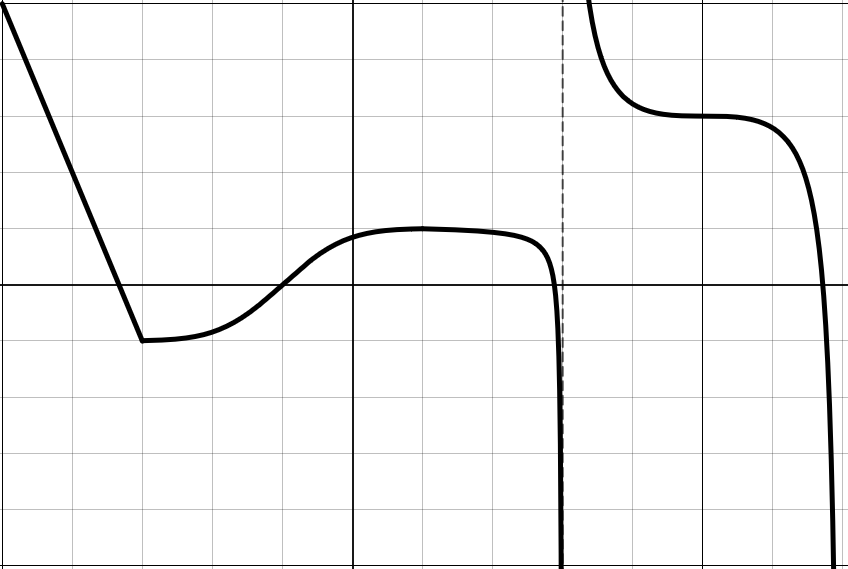
\includegraphics[width=0.85\textwidth]{../images/DFb-v1.png}    
\end{center}


Sketch the graph of $q'(x)$ on the blank axes below.

\begin{center}
    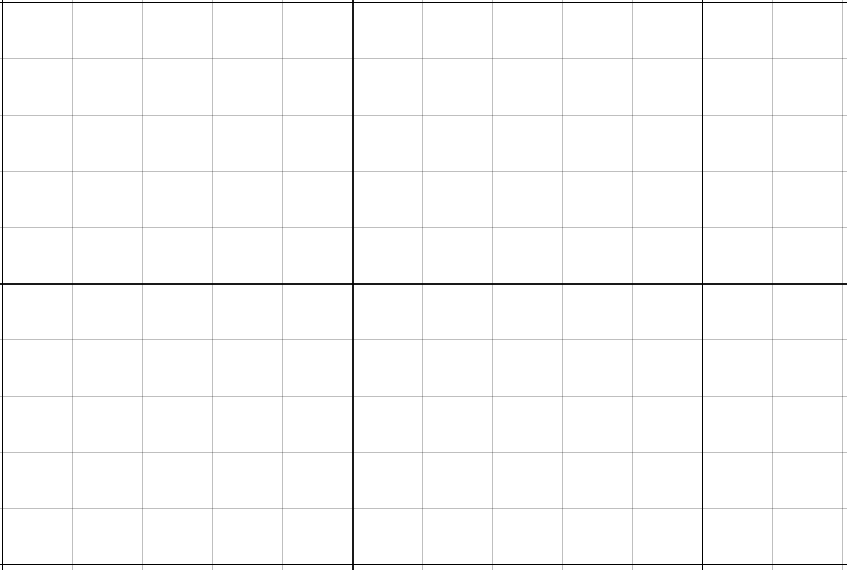
\includegraphics[width=0.85\textwidth]{../images/DFb-v1-blank.png}    
\end{center}

%%%%%%%%%%%%%%%%%%%%%%%%%%%%%%%%%%%%%%%%%%%%%%%%%%%%%%%%%
\pagebreak
%%%%%%%%%%%%%%%%%%%%%%%%%%%%%%%%%%%%%%%%%%%%%%%%%%%%%%%%%

\section{Learning target DFb, version 2}

Given a graph of a function, estimate specific values of the derivative, and/or produce a sketch of the derivative function.

\hrulefill

Here is the graph of some wacky function $h(t)$:

\begin{center}
    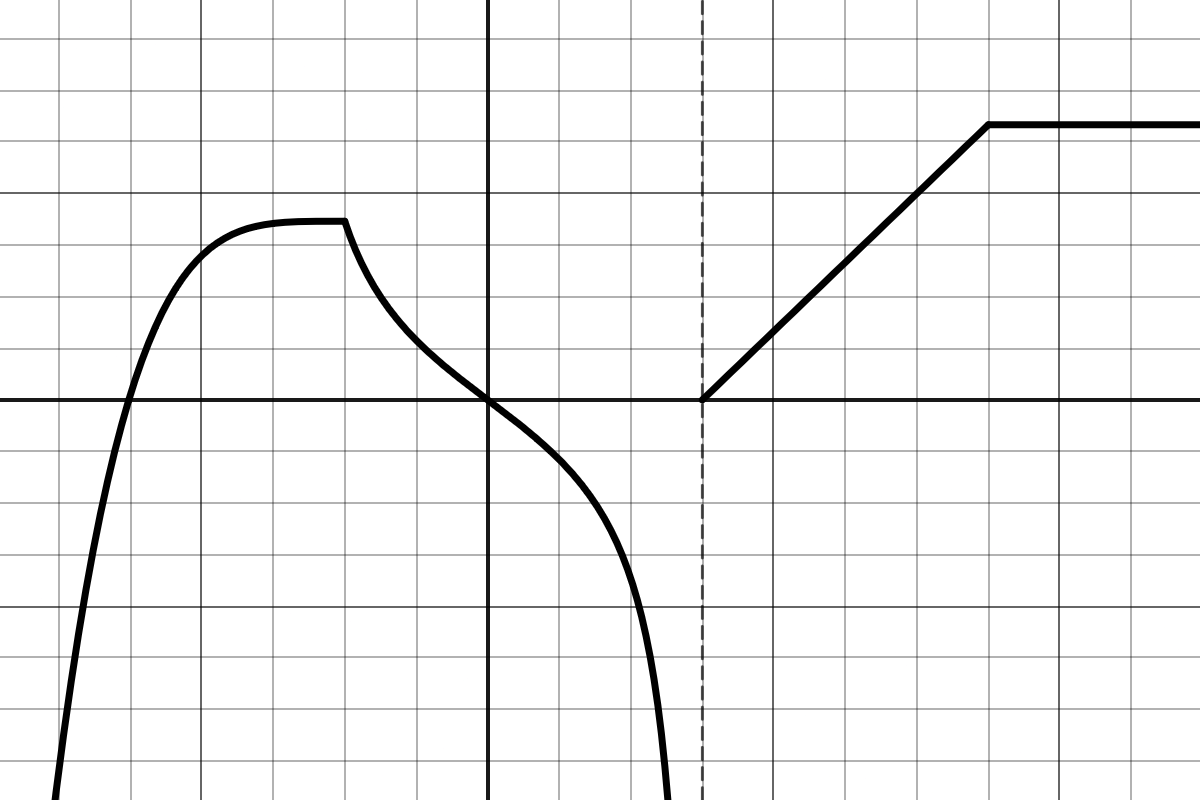
\includegraphics[width=0.85\textwidth]{../images/DFb-v2.png}    
\end{center}


Sketch the graph of $h'(t)$ on the blank axes below.

\begin{center}
    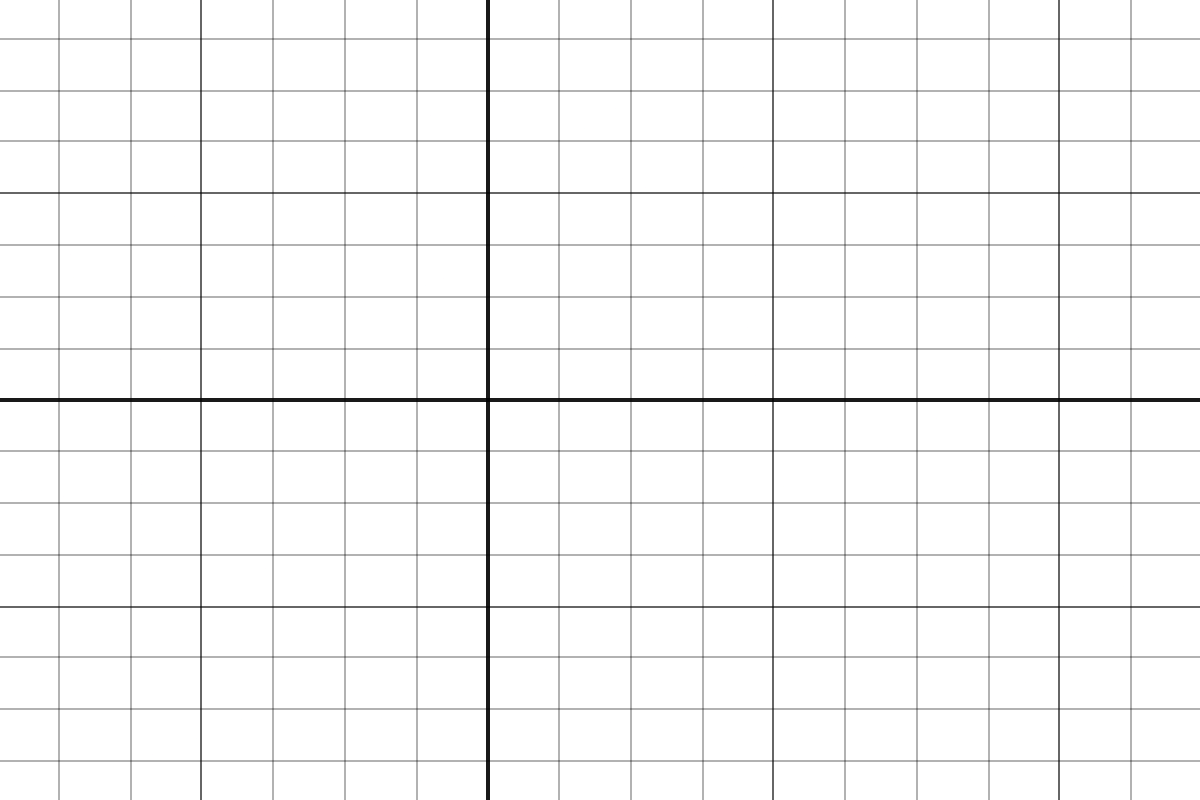
\includegraphics[width=0.85\textwidth]{../images/DFb-v2-blank.png}    
\end{center}

%%%%%%%%%%%%%%%%%%%%%%%%%%%%%%%%%%%%%%%%%%%%%%%%%%%%%%%%%
\pagebreak
%%%%%%%%%%%%%%%%%%%%%%%%%%%%%%%%%%%%%%%%%%%%%%%%%%%%%%%%%
\section{Learning target DFb, version 3}

Given a graph of a function, estimate specific values of the derivative, and/or produce a sketch of the derivative function.

\hrulefill

Here is the graph of some wacky function $z(x)$:

\begin{center}
    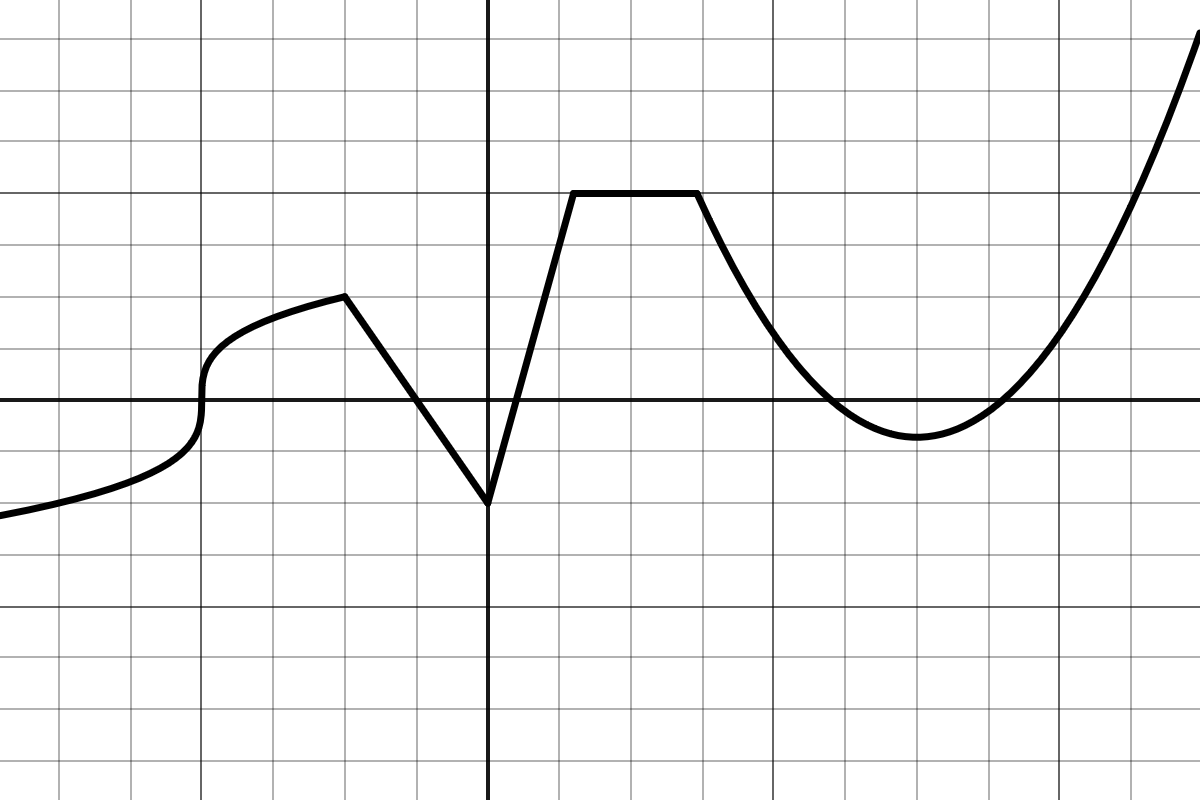
\includegraphics[width=0.85\textwidth]{../images/DFb-v3.png}    
\end{center}


Sketch the graph of $z'(x)$ on the blank axes below.

\begin{center}
    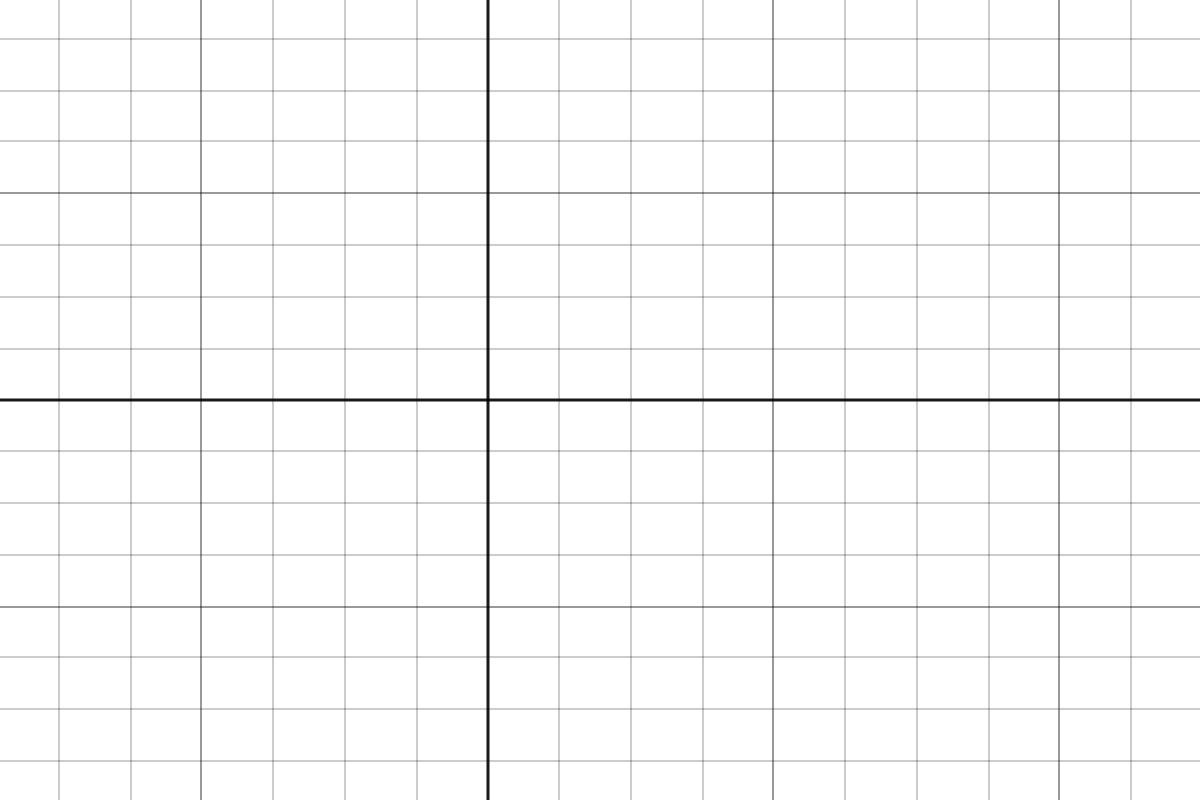
\includegraphics[width=0.85\textwidth]{../images/DFb-v3-blank.png}    
\end{center}

%%%%%%%%%%%%%%%%%%%%%%%%%%%%%%%%%%%%%%%%%%%%%%%%%%%%%%%%%
\pagebreak
%%%%%%%%%%%%%%%%%%%%%%%%%%%%%%%%%%%%%%%%%%%%%%%%%%%%%%%%%
\section{Learning target DFb, version 4}

Given a graph of a function, estimate specific values of the derivative, and/or produce a sketch of the derivative function.

\hrulefill

Here is the graph of some wacky function $g(t)$:

\begin{center}
    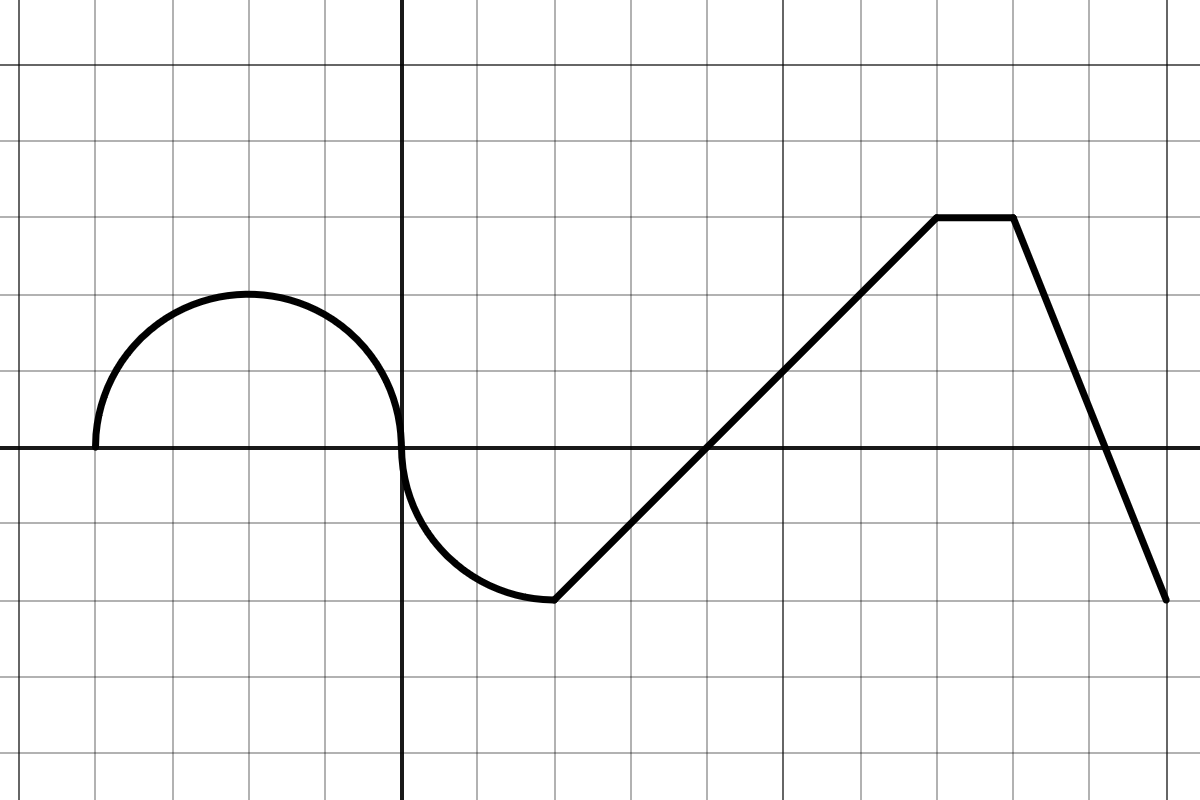
\includegraphics[width=0.85\textwidth]{../images/DFb-v4.png}    
\end{center}


Sketch the graph of $g'(t)$ on the blank axes below.

\begin{center}
    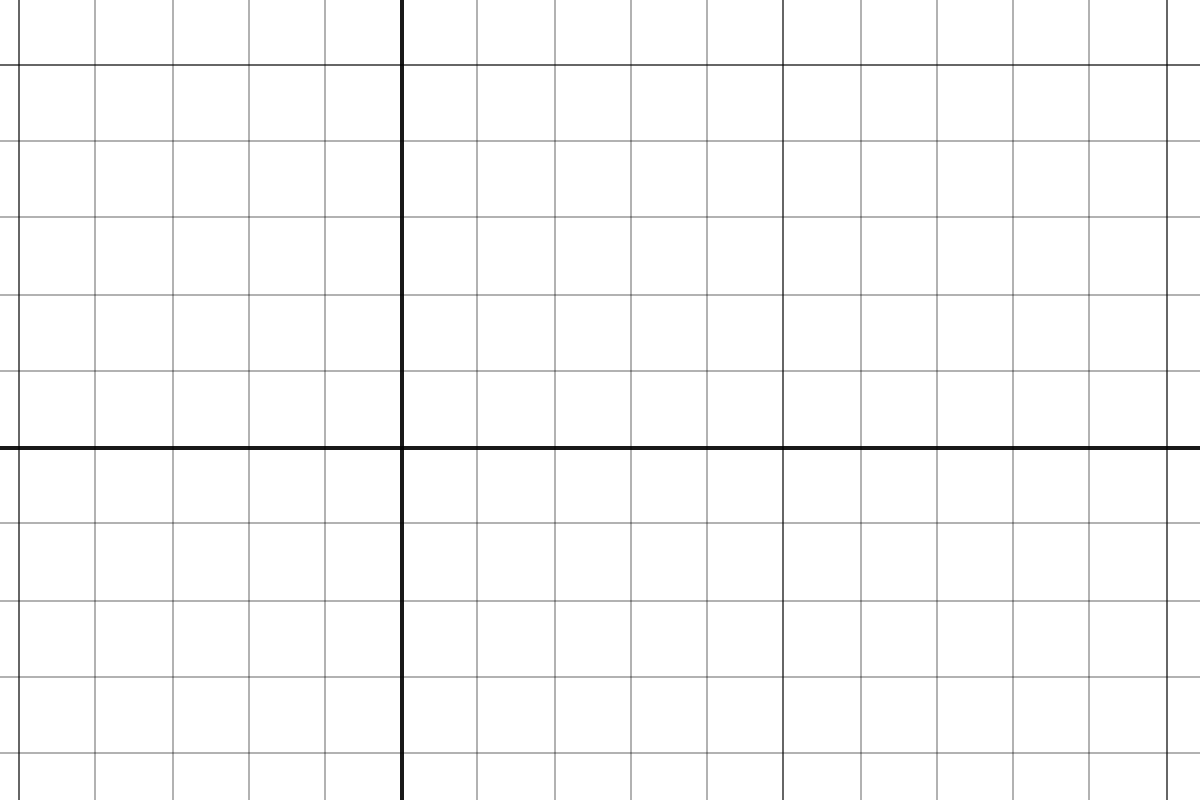
\includegraphics[width=0.85\textwidth]{../images/DFb-v4-blank.png}    
\end{center}

%%%%%%%%%%%%%%%%%%%%%%%%%%%%%%%%%%%%%%%%%%%%%%%%%%%%%%%%%
\pagebreak
%%%%%%%%%%%%%%%%%%%%%%%%%%%%%%%%%%%%%%%%%%%%%%%%%%%%%%%%%

\section{Learning target AD2, version 2}
Suppose that for some function \(p(x)\), you know the following information:
\begin{itemize}
    \item \(p(-2) = 5\),
    \item \(p'(-2) = 1.5\), 
    \item \(p''(x) < 0\) for \(x\)-values close to \(-2\). 
\end{itemize}

\begin{enumerate}[leftmargin=0pt]
    \item Explain and demonstrate how to find the linearization \(L(x)\) of \(p(x)\) at \(x =-2\). 
    \vfill
    \item Explain and demonstrate how to estimate the value of \(p(-2.03)\) using this linearization. 
    
    \vfill
    \item Is your estimate of \(p(-2.03)\) greater than or less than the actual value? How do you know?
    
    \vfill
    \item Sketch a possible graph of \(p(x)\) and its linearization \(L(x)\) nearby \(x =-2\) to illustrate your findings. Label important points in your sketch with their coordinates.
    
    \vfill
\end{enumerate}

%%%%%%%%%%%%%%%%%%%%%%%%%%%%%%%%%%%%%%%%%%%%%%%%%%%%%%%%%
\pagebreak
%%%%%%%%%%%%%%%%%%%%%%%%%%%%%%%%%%%%%%%%%%%%%%%%%%%%%%%%%

\section{Learning target AD2, version 3}

The funny thing about square roots is that most of the time, they are \textit{irrational} numbers, which means that they can't be written as fractions, and thus their decimal expansions go on forever and never repeat. For instance, \(\sqrt{67} = 8.18535277187244996995370372473392945888048681549803996306671520272366761446109794534392467163786834453471127515600621176294861011220414995972157\)

That is clearly not a particularly useful answer to the question ``what's \(\sqrt{67}\)?''
We might in particular prefer to come up with a \textit{fraction} that is a reasonably good approximation.

\begin{enumerate}[(a)]
	\item The number $\sqrt{67}$ is an output $y$-value of the function $f(x) = \sqrt{x}$. What's the corresponding input $x$-value?
	\vfill
	\item Think of an $x$-value that's close to the input value you said in part (a), but for which it is \textit{easy} to figure out the square root.

	$f(\underline{\qquad}) = \sqrt{\phantom{6464}} = \underline{\qquad}$

	\vfill
	\item Compute $f'(x)$ and plug in your easy $x$-value. Leave your answer as a fraction.

	$f'(\underline{\qquad}) = \underline{\qquad}$
	\vfill
	\item Write down the equation for the tangent line to $f(x)$ at the easy $x$-value.

	$L(x) =$
	\vfill
	\item Lastly but not leastly, plug in the hard $x$-value into the equation for the tangent line. Leave your answer as a fraction.
\end{enumerate}

%%%%%%%%%%%%%%%%%%%%%%%%%%%%%%%%%%%%%%%%%%%%%%%%%%%%%%%%%
\pagebreak
%%%%%%%%%%%%%%%%%%%%%%%%%%%%%%%%%%%%%%%%%%%%%%%%%%%%%%%%%

\section{Learning target AD2, version 4}

Part of the graph of this function $f(x)$ has been erased. 
We'll use linear approximation to recover the values.

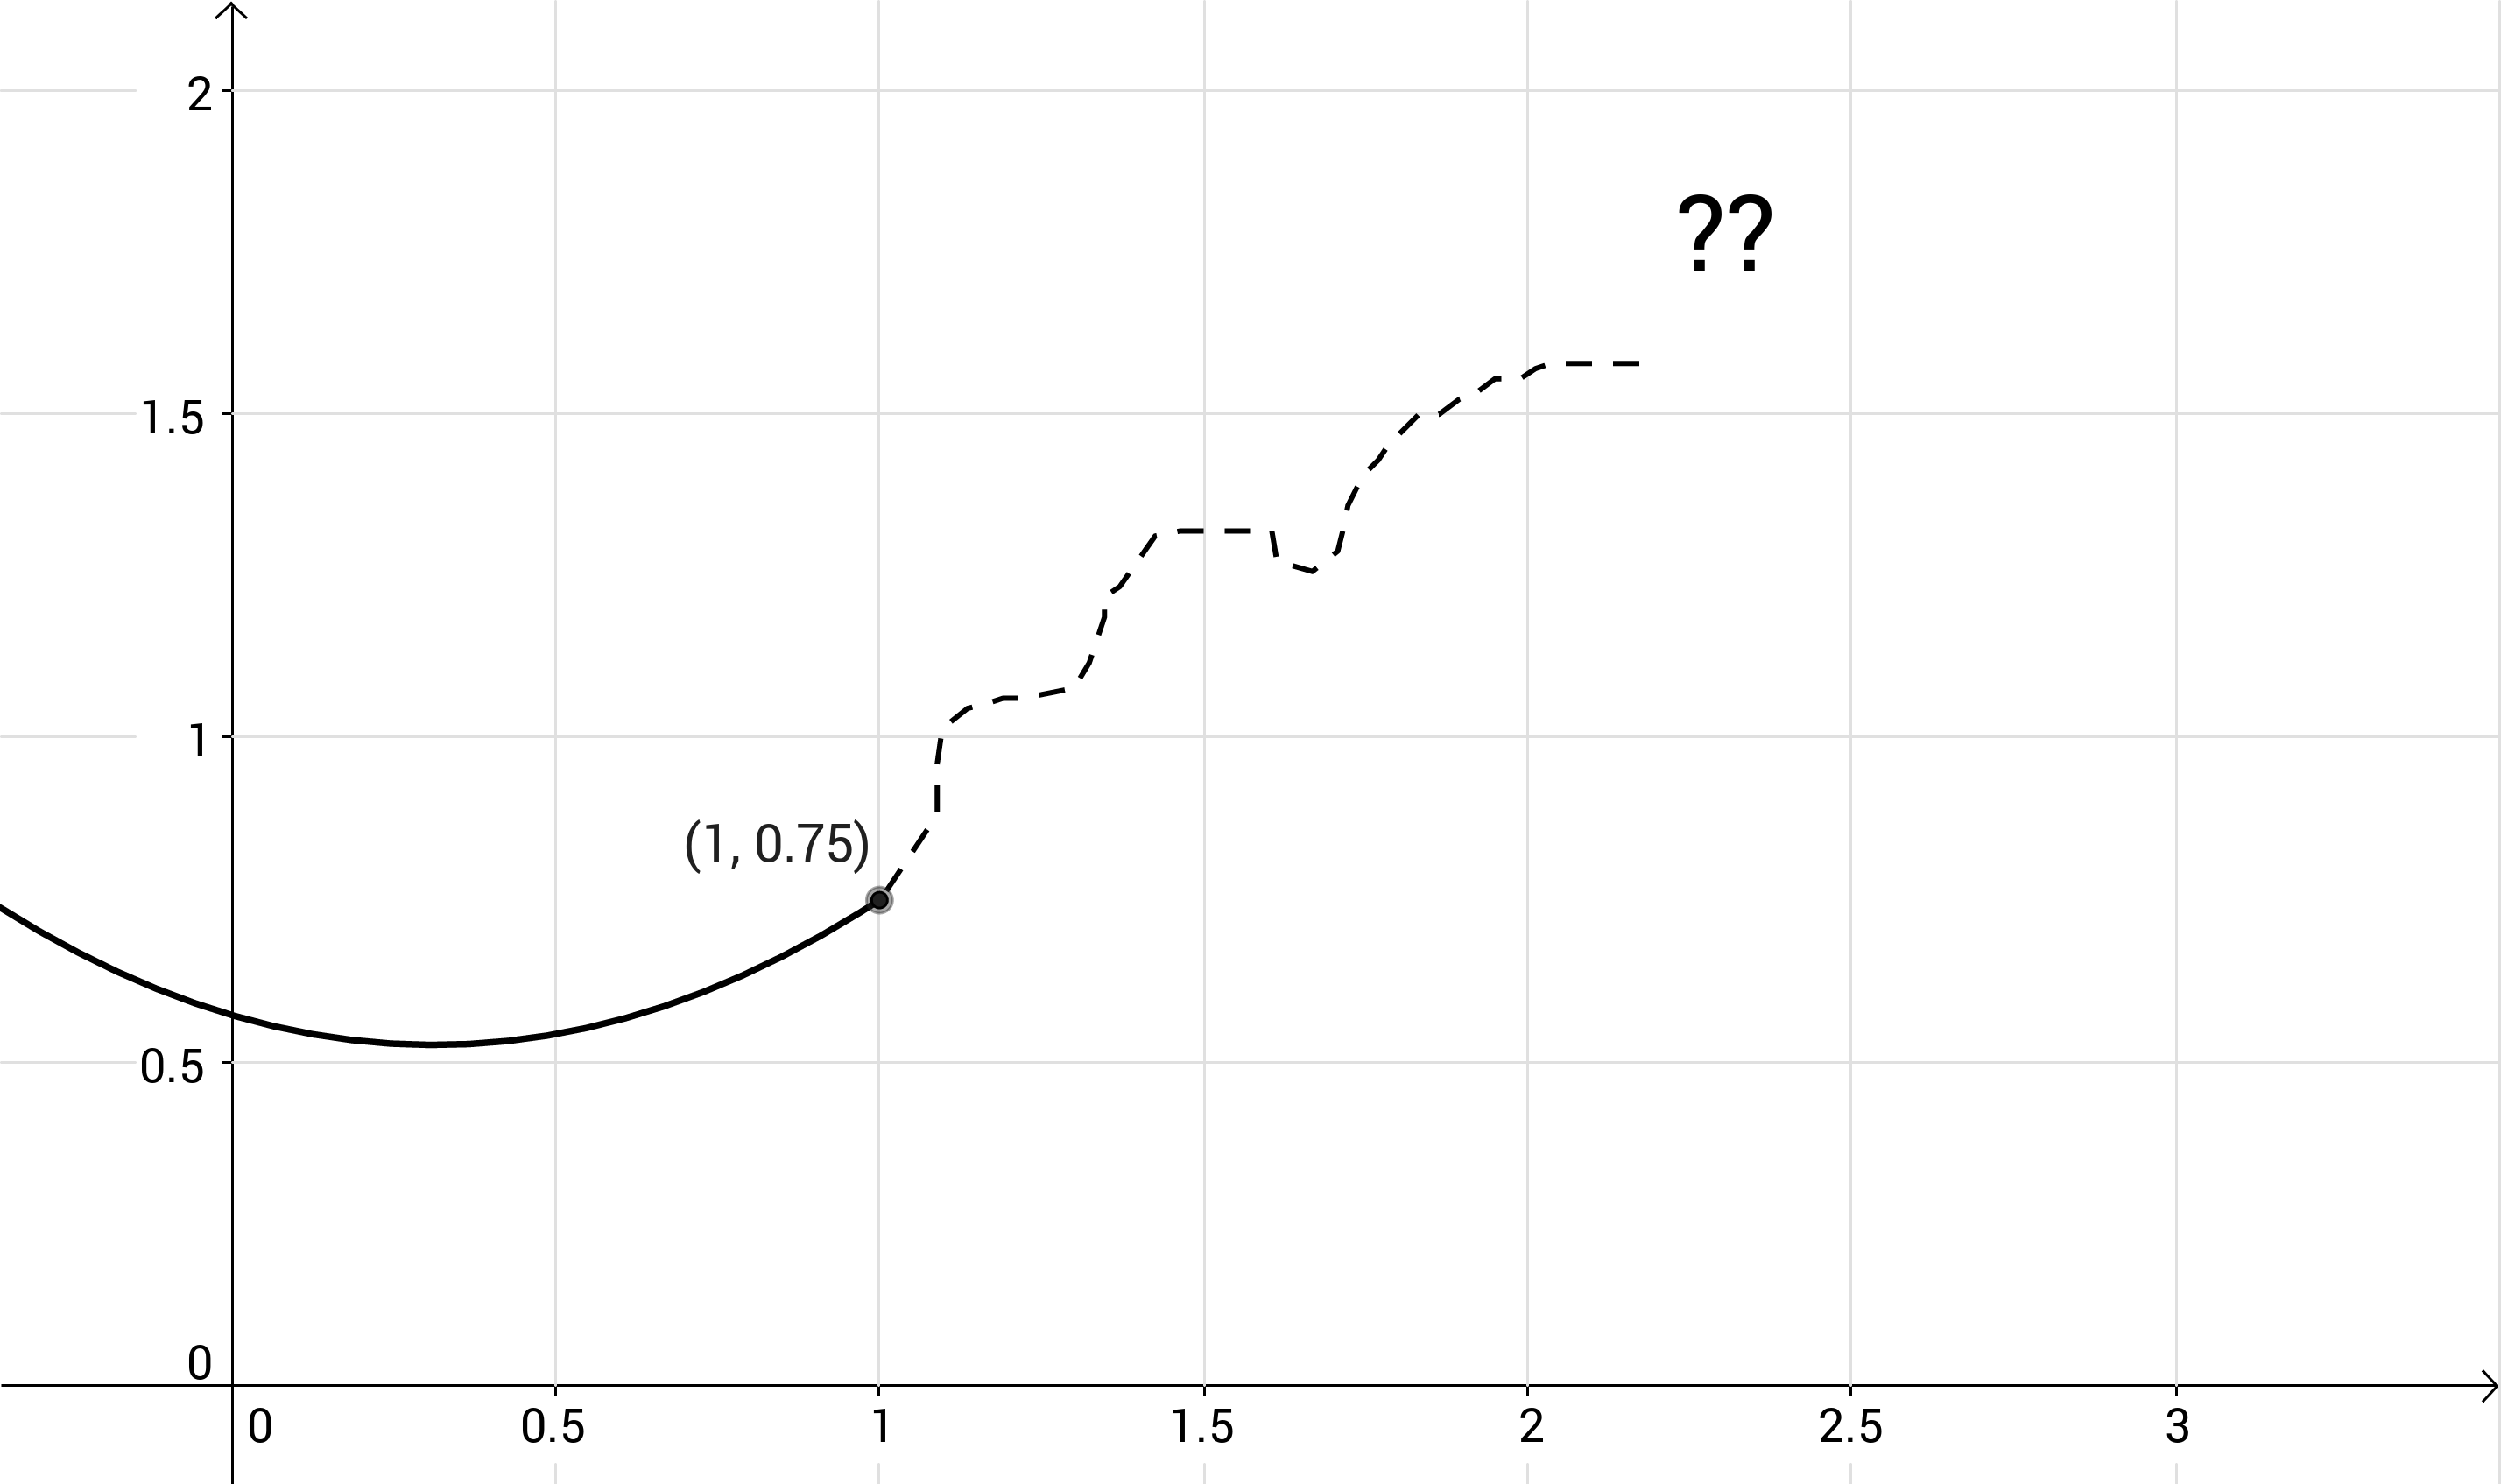
\includegraphics[width=\textwidth]{../images/linapprox.png}

\begin{enumerate}[(a)]
\item Draw the tangent line to this function at $x = 1$.
\item Suppose we know that $f'(1) = 0.65$. Use point-slope form to write down an equation for $L(x)$, the tangent line to this function at $x=1$.
\vfill
\item Use your equation for $L(x)$ to estimate $f(1.4)$.
\vfill
\item Do you think it is more likely that this is an 
overestimate or an underestimate? How come?
\vfill
\end{enumerate}

%%%%%%%%%%%%%%%%%%%%%%%%%%%%%%%%%%%%%%%%%%%%%%%%%%%%%%%%%
\pagebreak
%%%%%%%%%%%%%%%%%%%%%%%%%%%%%%%%%%%%%%%%%%%%%%%%%%%%%%%%%

\section{Learning target DF3, version 1}

Compute basic derivatives using algebraic rules.

\hrulefill

Demonstrate and explain how to find the derivative of the following functions. Be sure to write down which derivative rules (constant multiple, sum/difference, etc.) you are using in your work.

\begin{enumerate}
    \item \(f(x) = 2 \, \cos\left(x\right) + 4 \, e^{x}\) 
    \vfill
    \item \(h(t) = \sqrt[3]{t^4} + \frac{4}{t^{4}}\) \quad (Don't use the quotient rule or the chain rule.)
    \vfill
    \item \(g(w) = 6 \, w^{3} - 2 \, w^{2} - 9 \, w - 2\)
    \vfill
    \item \(C(t) = 64(e^7 + 7^e)- \dfrac{\sqrt[27]{193262}}{16-\pi^2} + \dfrac{67}{8675309}\) \quad
(Hint: Look carefully!)
\end{enumerate}



%%%%%%%%%%%%%%%%%%%%%%%%%%%%%%%%%%%%%%%%%%%%%%%%%%%%%%%%%
\pagebreak
%%%%%%%%%%%%%%%%%%%%%%%%%%%%%%%%%%%%%%%%%%%%%%%%%%%%%%%%%

\section{Learning target DF3, version 2}

Compute basic derivatives using algebraic rules.

\hrulefill

Demonstrate and explain how to find the derivative of the following functions. Be sure to write down which derivative rules (constant multiple, sum/difference, etc.) you are using in your work.

\begin{enumerate}
    \item \(g(t) = \sqrt[4]{t^3} + \frac{7}{t^{4}}\) \quad (Don't use the quotient rule or the chain rule.)
    \vfill
    \item \(f(x) = -x^{5} - 4 \, x^{4} + 5 \, x - 4\)
    \vfill
    \item \(h(y) = -4 \, \ln\left(y\right) + 3 \, \sin\left(y\right)\)
    \vfill
\end{enumerate}

%%%%%%%%%%%%%%%%%%%%%%%%%%%%%%%%%%%%%%%%%%%%%%%%%%%%%%%%%
\pagebreak
%%%%%%%%%%%%%%%%%%%%%%%%%%%%%%%%%%%%%%%%%%%%%%%%%%%%%%%%%

\section{Learning target DF3, version 3}

Compute basic derivatives using algebraic rules.

\hrulefill

Demonstrate and explain how to find the derivative of the following functions. Be sure to write down which derivative rules (constant multiple, sum/difference, etc.) you are using in your work.

\begin{enumerate}
    \item \(f(y) = -2 \, e^{y} - 4 \, \sin\left(y\right)\) 
    \vfill
    \item \(h(x) = 9 \, x^{5} - x^{4} - x^{3} - 6\) 
    \vfill
    \item \(g(t) = \sqrt[3]{t^7} + \frac{2}{t^{2}}\)  \quad (Don't use the quotient rule or the chain rule.)
    \vfill
\end{enumerate}

%%%%%%%%%%%%%%%%%%%%%%%%%%%%%%%%%%%%%%%%%%%%%%%%%%%%%%%%%
\pagebreak
%%%%%%%%%%%%%%%%%%%%%%%%%%%%%%%%%%%%%%%%%%%%%%%%%%%%%%%%%

\section{Learning target DF3, version 4}

Compute basic derivatives using algebraic rules.

\hrulefill

Demonstrate and explain how to find the derivative of the following functions. Be sure to write down which derivative rules (constant multiple, sum/difference, etc.) you are using in your work.

\begin{enumerate}
    \item \(g(t) = -5 \, t^{4} - 9 \, t^{3} - 6 \, t^{2} - 6\)
    \vfill
    \item \(f(w) = \sqrt[3]{w^5} + \frac{4}{w^{5}}\)  \quad (Don't use the quotient rule or the chain rule.)
    \vfill
    \item \(h(y) = 2 \, e^{y} + 2 \, \sin\left(y\right)\)
    \vfill
\end{enumerate}

%%%%%%%%%%%%%%%%%%%%%%%%%%%%%%%%%%%%%%%%%%%%%%%%%%%%%%%%%
\pagebreak
%%%%%%%%%%%%%%%%%%%%%%%%%%%%%%%%%%%%%%%%%%%%%%%%%%%%%%%%%

\section{Learning target DF4, version 1}

Compute derivatives using the Product and Quotient Rules.

\hrulefill

Demonstrate and explain how to find the derivative of the following functions. Be sure to write down which derivative rules (product, quotient, sum and difference, etc.) you are using.

\begin{enumerate}
    \item \(\renewcommand{\log}{\ln} g(x)= \frac{\log\left(x\right)}{2 \, x^{2} + 6 \, x - 3}\)
    \vfill
    \item \(\renewcommand{\log}{\ln} f(x)= {\left(x^{2} - 2 \, x - 4\right)} \cos\left(x\right)\)
    \vfill
    \item \(\renewcommand{\log}{\ln} h(t)= -\frac{3 \, t^{2} + 2 \, t + 3}{t^{3}}\)
    \vfill
\end{enumerate}



%%%%%%%%%%%%%%%%%%%%%%%%%%%%%%%%%%%%%%%%%%%%%%%%%%%%%%%%%
\pagebreak
%%%%%%%%%%%%%%%%%%%%%%%%%%%%%%%%%%%%%%%%%%%%%%%%%%%%%%%%%

\section{Learning target DF4, version 2}

Compute derivatives using the Product and Quotient Rules.

\hrulefill

Demonstrate and explain how to find the derivative of the following functions. Be sure to write down which derivative rules (product, quotient, sum and difference, etc.) you are using.

\begin{enumerate}
    \item \(\renewcommand{\log}{\ln} h(w)= -\frac{\cos\left(w\right)}{6 \, w^{2} + 5 \, w + 4}\)
    \vfill
    \item \( \renewcommand{\log}{\ln} g(w)= \frac{3 \, w^{2} + 5 \, w - 1}{w^{8}}\)
    \vfill
    \item \(\renewcommand{\log}{\ln} f(w)= -{\left(4 \, w^{2} + 6 \, w + 1\right)} \log\left(w\right)\)
    \vfill
\end{enumerate}

%%%%%%%%%%%%%%%%%%%%%%%%%%%%%%%%%%%%%%%%%%%%%%%%%%%%%%%%%
\pagebreak
%%%%%%%%%%%%%%%%%%%%%%%%%%%%%%%%%%%%%%%%%%%%%%%%%%%%%%%%%

\section{Learning target DF4, version 3}

Compute derivatives using the Product and Quotient Rules.

\hrulefill

Demonstrate and explain how to find the derivative of the following functions. Be sure to write down which derivative rules (product, quotient, sum and difference, etc.) you are using.

\begin{enumerate}
    \item \(\renewcommand{\log}{\ln} g(w)= -\frac{2 \, w^{2} + 6 \, w + 1}{w^{1/5}}\)
    \vfill
    \item \(\renewcommand{\log}{\ln} f(w)= -\frac{\sin\left(w\right)}{3 \, w^{2} - 3 \, w + 4}\)
    \vfill
    \item \(\renewcommand{\log}{\ln} h(w)= -{\left(2 \, w^{2} + 5 \, w - 5\right)} e^{w}\)
    \vfill
\end{enumerate}

%%%%%%%%%%%%%%%%%%%%%%%%%%%%%%%%%%%%%%%%%%%%%%%%%%%%%%%%%
\pagebreak
%%%%%%%%%%%%%%%%%%%%%%%%%%%%%%%%%%%%%%%%%%%%%%%%%%%%%%%%%

\section{Learning target DF4, version 4}

Compute derivatives using the Product and Quotient Rules.

\hrulefill

Demonstrate and explain how to find the derivative of the following functions. Be sure to write down which derivative rules (product, quotient, sum and difference, etc.) you are using.

\begin{enumerate}
    \item \(\renewcommand{\log}{\ln} f(x)= -{\left(3 \, x^{2} - 6 \, x + 2\right)} \cos\left(x\right)\)
    \vfill
    \item \(\renewcommand{\log}{\ln} h(y)= \frac{3 \, y^{2} - 3 \, y - 2}{\sin\left(y\right)}\)
    \vfill
    \item \(\renewcommand{\log}{\ln} g(w)= \frac{2 \, w^{2} - w + 4}{w^{1/6}}\)
    \vfill
\end{enumerate}

%%%%%%%%%%%%%%%%%%%%%%%%%%%%%%%%%%%%%%%%%%%%%%%%%%%%%%%%%
\pagebreak
%%%%%%%%%%%%%%%%%%%%%%%%%%%%%%%%%%%%%%%%%%%%%%%%%%%%%%%%%

\section{Learning target DF5, version 1}

Compute derivatives using the Chain Rule.

\hrulefill

Demonstrate and explain how to find the derivative of the following functions. Be sure to write down which derivative rules (chain, product, quotient, sum and difference, etc.) you are using.

\begin{enumerate}
    \item \(h(t)= 16 \, {\left(t + e^{t} + 2\right)}^{4}\)
    \vfill
    \item \(f(w)= 5 \, \sin\left(w^{\frac{7}{3}}\right)\)
    \vfill
    \item \(g(x)= 5 \, \Big(\sin\left(x\right)\Big)^{\frac{7}{3}}\)
    \vfill
    \item \(p(y) = 2\ln\left(\sin(y) + y^2 + 3\right)\)
    \vfill
\end{enumerate}



%%%%%%%%%%%%%%%%%%%%%%%%%%%%%%%%%%%%%%%%%%%%%%%%%%%%%%%%%
\pagebreak
%%%%%%%%%%%%%%%%%%%%%%%%%%%%%%%%%%%%%%%%%%%%%%%%%%%%%%%%%

\section{Learning target DF5, version 2}

Compute derivatives using the Chain Rule.

\hrulefill

Demonstrate and explain how to find the derivative of the following functions. Be sure to write down which derivative rules (chain, product, quotient, sum and difference, etc.) you are using.

\begin{enumerate}
    \item \(h(x)= -9 \, \cos\left(-5 \, x^{2} + 3 \, x + 4\right)\)
    \vfill
    \item \(f(y)= -9 \, \sin\left(y^{7/2}\right)\)
    \vfill
    \item \(g(t)= -9 \, \Big(\sin\left(t\right)\Big)^{7/2}\)
    \vfill
    \item \(k(w)= {\left(3 \, w + e^{w} - 1\right)}^{4}\)
    \vfill
\end{enumerate}

%%%%%%%%%%%%%%%%%%%%%%%%%%%%%%%%%%%%%%%%%%%%%%%%%%%%%%%%%
\pagebreak
%%%%%%%%%%%%%%%%%%%%%%%%%%%%%%%%%%%%%%%%%%%%%%%%%%%%%%%%%

\section{Learning target DF5, version 3}

Compute derivatives using the Chain Rule.

\hrulefill

Demonstrate and explain how to find the derivative of the following functions. Be sure to write down which derivative rules (chain, product, quotient, sum and difference, etc.) you are using.

\begin{enumerate}
    \item \(k(w)= -{\left(5 \, w + 2 \, e^{w} + 1\right)}^{3}\)
    \vfill
    \item \(g(y)= 3 \, \sin\left(y^{2/5}\right)\)
    \vfill
    \item \(h(x)= 6 \, \cos\left(-5 \, x^{2} - x + 4\right)\)
    \vfill
    \item \(f(t)= 3 \, \Big(\sin\left(t\right)\Big)^{2/5}\)
    \vfill
\end{enumerate}

%%%%%%%%%%%%%%%%%%%%%%%%%%%%%%%%%%%%%%%%%%%%%%%%%%%%%%%%%
\pagebreak
%%%%%%%%%%%%%%%%%%%%%%%%%%%%%%%%%%%%%%%%%%%%%%%%%%%%%%%%%

\section{Learning target DF5, version 4}

Compute derivatives using the Chain Rule.

\hrulefill

Demonstrate and explain how to find the derivative of the following functions. Be sure to write down which derivative rules (chain, product, quotient, sum and difference, etc.) you are using.

\begin{enumerate}
    \item \(g(t)= 3 \, \cos\left(-3 \, t^{2} - 3 \, t + 4\right)\)
    \vfill
    \item \(h(y)= 5 \, \sin\left(y^{7/2}\right)\)
    \vfill
    \item \(k(w)= 5 \, \Big(\sin\left(w\right)\Big)^{7/2}\)
    \vfill
    \item \(f(x)= -{\left(5 \, x + 3 \, e^{x} - 4\right)}^{5}\)
    \vfill
\end{enumerate}

%%%%%%%%%%%%%%%%%%%%%%%%%%%%%%%%%%%%%%%%%%%%%%%%%%%%%%%%%
\pagebreak
%%%%%%%%%%%%%%%%%%%%%%%%%%%%%%%%%%%%%%%%%%%%%%%%%%%%%%%%%

\section{Learning target DF6, version 1}

Compute derivatives of complicated functions using a combination of derivative rules.

\hrulefill

Demonstrate and explain how to find the derivative of the following functions. Be sure to write down which derivative rules (chain, product, quotient, sum and difference, etc.) you are using.

\begin{enumerate}
    \item \(g(x) = \sqrt{\cos\left(-2 \, x^{4} + 5\right)}\)
    \vfill
    \item \(f(w) = \left( \frac{6 \, w^{6} - 1}{5 \, w + 3} \right)^{ 4 }\)
    \vfill
    \item \(h(y) = {\left(3 \, y^{2} + 7 \, y\right)}^{4}\cdot y^{1/4}\)
    \vfill
\end{enumerate}



%%%%%%%%%%%%%%%%%%%%%%%%%%%%%%%%%%%%%%%%%%%%%%%%%%%%%%%%%
\pagebreak
%%%%%%%%%%%%%%%%%%%%%%%%%%%%%%%%%%%%%%%%%%%%%%%%%%%%%%%%%

\section{Learning target DF6, version 2}

Compute derivatives of complicated functions using a combination of derivative rules.

\hrulefill

Demonstrate and explain how to find the derivative of the following functions. Be sure to write down which derivative rules (chain, product, quotient, sum and difference, etc.) you are using.

\begin{enumerate}
    \item \(f(w) = \left( \frac{5 \, w^{6} + 1}{6w^5 + 2} \right)^{ 6 }\)
    \vfill
    \item \(g(x) = {\left(5 \, x^{5} - 2 \, x^{3}\right)}^{6}\cdot  \sqrt{x}\)
    \vfill
    \item \(h(y) = \sqrt{\sin\left(-2 \, y^{4} + 4\right)}\)
    \vfill
\end{enumerate}

%%%%%%%%%%%%%%%%%%%%%%%%%%%%%%%%%%%%%%%%%%%%%%%%%%%%%%%%%
\pagebreak
%%%%%%%%%%%%%%%%%%%%%%%%%%%%%%%%%%%%%%%%%%%%%%%%%%%%%%%%%

\section{Learning target DF6, version 3}

Compute derivatives of complicated functions using a combination of derivative rules.

\hrulefill

Demonstrate and explain how to find the derivative of the following functions. Be sure to write down which derivative rules (chain, product, quotient, sum and difference, etc.) you are using.

\begin{enumerate}
    \item \(f(t) = \sqrt{\cos\left(-t^{4} - 6\right)}\)
    \vfill
    \item \(h(x) = \left( \frac{5 \, x^{5} - 2}{3 x^{3} - 1} \right)^{ 4 }\)
    \vfill
    \item \(g(w) = {\left(3 \, w^{3} + 2 \, w^{2}\right)}^{3} \cdot w^{2/3}\)
    \vfill
\end{enumerate}

%%%%%%%%%%%%%%%%%%%%%%%%%%%%%%%%%%%%%%%%%%%%%%%%%%%%%%%%%
\pagebreak
%%%%%%%%%%%%%%%%%%%%%%%%%%%%%%%%%%%%%%%%%%%%%%%%%%%%%%%%%

\section{Learning target DF6, version 4}

Compute derivatives of complicated functions using a combination of derivative rules.

\hrulefill

Demonstrate and explain how to find the derivative of the following functions. Be sure to write down which derivative rules (chain, product, quotient, sum and difference, etc.) you are using.

\begin{enumerate}
    \item \(h(t) = \sqrt{\cos\left(-4 \, t^{3} - t\right)}\)
    \vfill
    \item \(g(w) = {\left(5 \, w^{3} + 7 \, w^{2}\right)}^{3} \cdot \sqrt{w}\)
    \vfill
    \item \(f(y) = \left(\frac{y^{2} - 5}{3 \, y^{3} + 4} \right)^{ 5 }\)
    \vfill
\end{enumerate}

%%%%%%%%%%%%%%%%%%%%%%%%%%%%%%%%%%%%%%%%%%%%%%%%%%%%%%%%%
\pagebreak
%%%%%%%%%%%%%%%%%%%%%%%%%%%%%%%%%%%%%%%%%%%%%%%%%%%%%%%%%

\section{Learning target DF7, version 1}

Compute derivatives of implicitly-defined functions.

\hrulefill

Consider the curve defined implicitly by the equation
	$$xy^3 + 2xy = 6$$
	
	\begin{enumerate}[leftmargin=15pt]
	
		\item Use implicit differentiation to find an expression for $\frac{dy}{dx}$ that depends on $x$ and $y$.  Show all of your work and thinking clearly, using correct notation.

		\vfill
	
		
		\item Notice that the point $(2,1)$ lies on the curve $xy^3 + 2xy = 6$.  Find the exact slope of the tangent line to the curve at $(2,1)$.  Show clearly how you determined this value, and label your work with proper notation.
		
		\vfill
	
	\end{enumerate}

%%%%%%%%%%%%%%%%%%%%%%%%%%%%%%%%%%%%%%%%%%%%%%%%%%%%%%%%%
\pagebreak
%%%%%%%%%%%%%%%%%%%%%%%%%%%%%%%%%%%%%%%%%%%%%%%%%%%%%%%%%

\section{Learning target DF7, version 2}

Compute derivatives of implicitly-defined functions.

\hrulefill

The equation \(x^{3}-y^{3}=9xy\) makes a curve called the \textit{folium of Descartes}.

\begin{enumerate}
	\item Use implicit differentiation to find an expression for $\frac{dy}{dx}$ that depends on $x$ and $y$.  Show all of your work and thinking clearly, using correct notation.

	\vfill

	\item Find the exact slope of the tangent line to this curve at the point \((-2, 4)\). Show clearly how you determined this value, and label your work with proper notation.

	\vfill

	\item (Also AD2) Find an equation for the tangent line to this curve at this point, and use your tangent line to make a reasonable guess about the $y$-coordinate of the point $(-2.5, \rule{0.75cm}{0.15mm} )$.
	\vspace{1in}
\end{enumerate}

%%%%%%%%%%%%%%%%%%%%%%%%%%%%%%%%%%%%%%%%%%%%%%%%%%%%%%%%%
\pagebreak
%%%%%%%%%%%%%%%%%%%%%%%%%%%%%%%%%%%%%%%%%%%%%%%%%%%%%%%%%

\section{Learning target DF7, version 3}

Compute derivatives of implicitly-defined functions.

\hrulefill

Consider the curve defined implicitly by the equation
\[x^5 - 8\, y^4 = \sin\left(y\right) - 7.\]

\begin{enumerate}[(a)]
	\item Use implicit differentiation to find an expression for $\frac{dy}{dx}$ that depends on $x$ and $y$.  Show all of your work and thinking clearly, using correct notation.

	\vfill

	\item This curve contains the point \((-1.4758, 0)\) (or, pretty close to that). Find the exact slope of the tangent line to this curve at this point. Show clearly how you determined this value, and label your work with proper notation.

	\vfill
\end{enumerate}

%%%%%%%%%%%%%%%%%%%%%%%%%%%%%%%%%%%%%%%%%%%%%%%%%%%%%%%%%
\pagebreak
%%%%%%%%%%%%%%%%%%%%%%%%%%%%%%%%%%%%%%%%%%%%%%%%%%%%%%%%%

\section{Learning target DF7, version 4}

Compute derivatives of implicitly-defined functions.

\hrulefill

Consider the curve defined implicitly by the equation
\[\sin(x+y) + \cos(x-y) = 1.\]

\begin{enumerate}[(a)]
	\item Use implicit differentiation to find an expression for $\frac{dy}{dx}$ that depends on $x$ and $y$.  Show all of your work and thinking clearly, using correct notation.

	\vfill

	\item This curve contains the point \(\left(\dfrac\pi{2},\dfrac\pi{2}\right)\). Find the exact slope of the tangent line to this curve at this point. Show clearly how you determined this value, and label your work with proper notation.

	\vfill
\end{enumerate}
%%%%%%%%%%%%%%%%%%%%%%%%%%%%%%%%%%%%%%%%%%%%%%%%%%%%%%%%%
\pagebreak
%%%%%%%%%%%%%%%%%%%%%%%%%%%%%%%%%%%%%%%%%%%%%%%%%%%%%%%%%

\section{Learning target AD3, version 1}

A wizard is developing a shrinking spell, but he needs to make sure it will work with his pointy hat, which is a cone whose height is three times its radius. Once he casts the spell, the height of his hat shrinks by 2 inches every second. How fast is the volume of his hat changing when the hat is just 3 inches tall? Give units on your answer.

\vspace{1em}

{\tiny Hints: Draw three pictures, label variables and constants, write down what you know and what you want to know, relate the variables, find the derivative wrt time, substitute and solve. 

The volume of a cone is a third of the volume of the cylinder that contains it: $V = 1/3 \cdot \pi r^2 h$.}

%%%%%%%%%%%%%%%%%%%%%%%%%%%%%%%%%%%%%%%%%%%%%%%%%%%%%%%%%
\pagebreak
%%%%%%%%%%%%%%%%%%%%%%%%%%%%%%%%%%%%%%%%%%%%%%%%%%%%%%%%%

\section{Learning target AD3, version 2}

Suppose an oil spill in the ocean formed a circle and was growing at a rate of \(53\) feet\(^2/\)minute. When the oil spill reaches a radius of \(35\) feet, how fast is the radius of the oil spill growing? 

\vspace{1em}

Make sure to do all six steps of the appropriate recipe.


%%%%%%%%%%%%%%%%%%%%%%%%%%%%%%%%%%%%%%%%%%%%%%%%%%%%%%%%%
\pagebreak
%%%%%%%%%%%%%%%%%%%%%%%%%%%%%%%%%%%%%%%%%%%%%%%%%%%%%%%%%
\section{Learning target AD3, version 3}


Gravel is being dumped from a conveyor belt at a rate of 12 cubic feet per minute. The gravel forms a pile in the shape of a right circular cone whose base diameter and height are always the same. How fast is the height of the pile increasing when the pile is 12 ft high? 
%%%%%%%%%%%%%%%%%%%%%%%%%%%%%%%%%%%%%%%%%%%%%%%%%%%%%%%%%
\pagebreak
%%%%%%%%%%%%%%%%%%%%%%%%%%%%%%%%%%%%%%%%%%%%%%%%%%%%%%%%%

\section{Learning target AD5 and AD4, version 1}

AD5: Draw annotated number lines and apply Derivative Tests to classify the critical points as local extrema.

AD4: Use the Extreme Value Theorem to find the global maximum and minimum values of a continuous function on a closed interval.

\hrulefill (AD5)

Consider the function
\(f(x)=2x^{3}+24x^{2}-54x+7\).
	
	\begin{enumerate}[leftmargin=15pt]

		\item Find the critical points using algebra, and draw a sign chart (aka labeled number line). \\
		Use the sign chart to decide what kind of extremum happens at each critical number.

		\vfill
		\vfill
	
		\hrulefill (AD4)
		\item Restricting the domain of this function to the interval $[-8, 2]$, what are the absolute maximum and absolute minimum values of this function, and where do they occur?

		\vfill
	
		
		\item What if we change the domain to $[-10, 2]$?
		
		\vfill
	
	\end{enumerate}

%%%%%%%%%%%%%%%%%%%%%%%%%%%%%%%%%%%%%%%%%%%%%%%%%%%%%%%%%%%%%%%%%%%%
\pagebreak
%%%%%%%%%%%%%%%%%%%%%%%%%%%%%%%%%%%%%%%%%%%%%%%%%%%%%%%%%%%%%%%%%%%%

\section{Learning target AD5 and AD4, version 2}

AD5: Draw annotated number lines and apply Derivative Tests to classify the critical points as local extrema.

AD4: Use the Extreme Value Theorem to find the global maximum and minimum values of a continuous function on a closed interval.

\hrulefill (AD5)

Consider the function
\(g(x) =-2x^{3}+18x^{2}+42x-100\).
	
	\begin{enumerate}[leftmargin=15pt]

		\item Find the critical numbers using algebra, and draw a sign chart (aka labeled number line). \\
		Use the sign chart to decide what kind of extremum happens at each critical number.

		\vfill
		\vfill
	
		\hrulefill (AD4)
		\item Restricting the domain of this function to the interval $[-4, 4]$, what are the absolute maximum and absolute minimum values of this function, and where do they occur?

		\vfill
	
		
		\item What if we change the domain to $[-4,10]$?
		
		\vfill
	
	\end{enumerate}
%%%%%%%%%%%%%%%%%%%%%%%%%%%%%%%%%%%%%%%%%%%%%%%%%%%%%%%%%%%%%%%%%%%%
\pagebreak
%%%%%%%%%%%%%%%%%%%%%%%%%%%%%%%%%%%%%%%%%%%%%%%%%%%%%%%%%%%%%%%%%%%%

\section{Learning target AD8, version 1}

Model and analyze scenarios using applied optimization.

{\tiny Hints: Draw three pictures; label variables and constants; write a constraint equation; write an objective function that just has one variable; find any endpoints; do the finding extrema recipe.}

\hrulefill

You are a dinosaur rancher, and you need to build pens for your three dinosaurs. You decide to build an electric fence around a rectangular region with total area of 25 square kilometers, and then separate this region into three equal-size rectangular pens with two more strips of electric fence. What's the minimum length of electric fencing you need to do this? 

\vspace{1em}

%Make sure to do all six steps of the appropriate recipe. 
Here is one of your three pictures.
\[
	\begin{tabular}{|l|c|c|}
		\hline
 		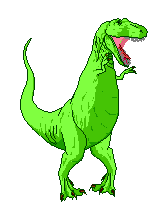
\includegraphics[width=1in]{../images/t-rex.png} & 
 		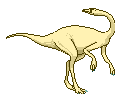
\includegraphics[width=1in]{../images/dromiceiomimus.png} &
 		
\includegraphics[width=1in]{../images/utahraptor.png} \\
		\hline
		% I need a padding row
		\multicolumn{1}{l}{} & \multicolumn{1}{l}{} & \multicolumn{1}{l}{} 
	\end{tabular}
\]
\vfill



The minimum length of fence is $\underbrace{\qquad\qquad}_{\text{number}}$ $\underbrace{\quad}_{\text{units}}$, 

and the dimensions of the dinosaur pen that make this work are 
$\underbrace{\qquad\qquad}_{\text{number}}\, 
\underbrace{\quad}_{\text{units}}
\times 
\underbrace{\qquad\qquad}_{\text{number}}\,
\underbrace{\quad}_{\text{units}}$.

%%%%%%%%%%%%%%%%%%%%%%%%%%%%%%%%%%%%%%%%%%%%%%%%%%%%%%%%%
\pagebreak
%%%%%%%%%%%%%%%%%%%%%%%%%%%%%%%%%%%%%%%%%%%%%%%%%%%%%%%%%


\section{Learning target AD8, version 2}

Model and analyze scenarios using applied optimization.

\hrulefill

If you take a regular 8.5" x 11" sheet of paper and cut squares out of the corners, you can fold up the flaps on all four sides to make a box (without a lid). How large should you cut the squares so that the resulting box has maximum volume?

{\tiny Hints: Draw three pictures; label variables and constants; write a constraint equation; write an objective function that just has one variable; find any endpoints; do the finding extrema recipe.}

\vfill

The maximum volume is $\underbrace{\qquad\qquad}_{\text{number}}$ $\underbrace{\quad}_{\text{units}}$, 

and the dimensions of the box that make this work are 
$\underbrace{\qquad\qquad}_{\text{number}}\, 
\underbrace{\quad}_{\text{units}}
\times 
\underbrace{\qquad\qquad}_{\text{number}}\,
\underbrace{\quad}_{\text{units}}
\times
\underbrace{\qquad\qquad}_{\text{number}}\,
\underbrace{\quad}_{\text{units}}$.

%%%%%%%%%%%%%%%%%%%%%%%%%%%%%%%%%%%%%%%%%%%%%%%%%%%%%%%%%
\pagebreak
%%%%%%%%%%%%%%%%%%%%%%%%%%%%%%%%%%%%%%%%%%%%%%%%%%%%%%%%%

\section{Learning target IN1, version 1}

Use geometric formulas to find definite integrals.

\hrulefill

Here is the graph of a function $h(t)$, which is made up of only straight lines and parts of circles.

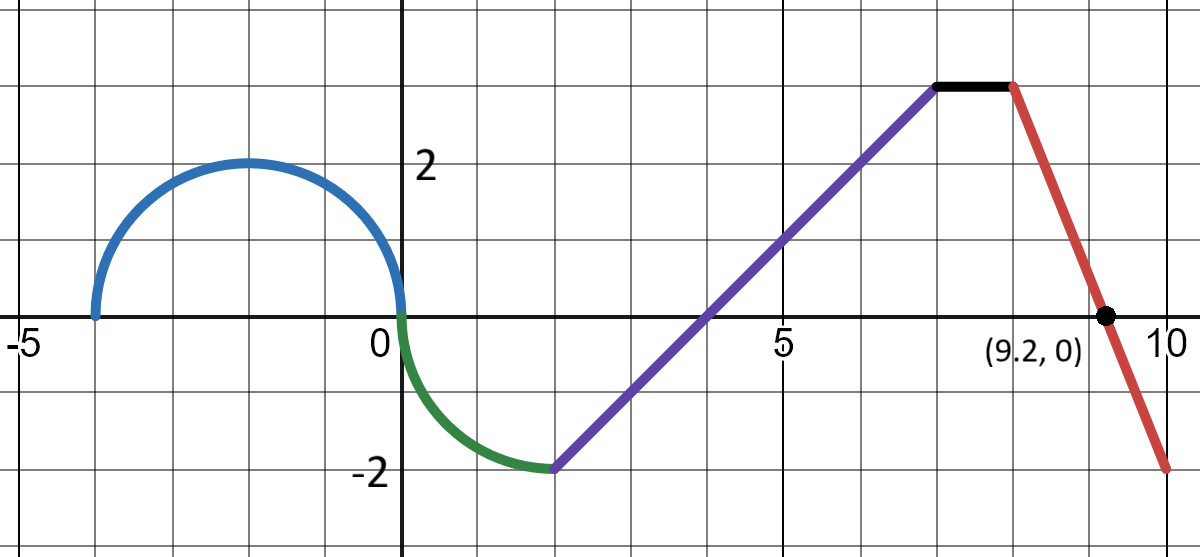
\includegraphics[width=\textwidth]{../images/IN1-v1.png}

Compute each of the following.

\begin{multicols*}{2}
{\everymath{\displaystyle}
\begin{enumerate}[(a)]
    \item $\int_{-4}^0 h(t)\, dt$

    \vfill
    \item $\int_0^2 h(t)\, dt$

    \vfill
    \item $\int_2^4 h(t)\, dt$

    \vfill
    \item $\int_4^7 h(t)\, dt$

    \vfill
    \columnbreak
    \item $\int_7^8 h(t)\, dt$

    \vfill
    \item $\int_8^{9.2} h(t)\, dt$

    \vfill
    \item $\int_{9.2}^{10} h(t)\, dt$

    \vfill
    \item $\int_{-4}^{10} h(t)\, dt$

\end{enumerate}
}
\end{multicols*}
%%%%%%%%%%%%%%%%%%%%%%%%%%%%%%%%%%%%%%%%%%%%%%%%%%%%%%%%%
\pagebreak
%%%%%%%%%%%%%%%%%%%%%%%%%%%%%%%%%%%%%%%%%%%%%%%%%%%%%%%%%

\section{Learning target IN1, version 2}

Use geometric formulas to find definite integrals.

\hrulefill

Here is the graph of a function $g(x)$, which is made up of only straight lines and parts of circles.

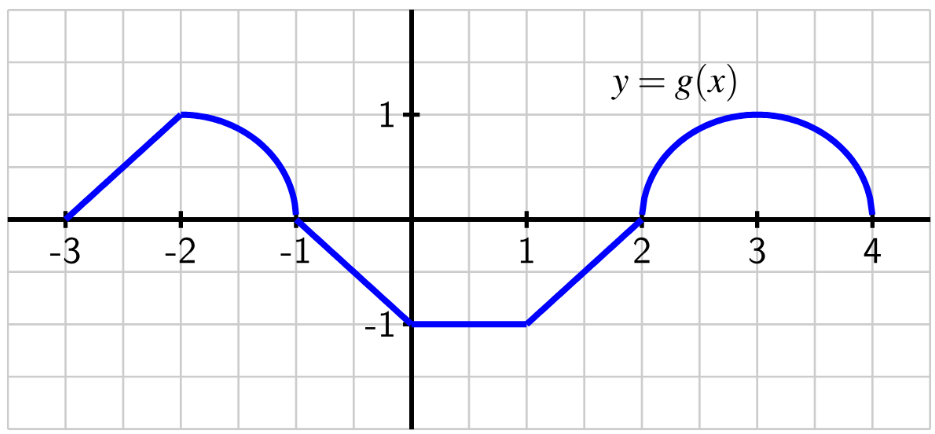
\includegraphics[width=\textwidth]{../images/IN1-v2.png}

Compute each of the following.

\begin{multicols*}{2}
{\everymath{\displaystyle}
\begin{enumerate}[(a)]
    \item $\int_{-3}^{-2} g(x)\ dx$

    \vfill
    \item $\int_{-2}^{-1} g(x)\ dx$

    \vfill
    \item $\int_{-1}^0 g(x)\ dx$

    \vfill
    \item $\int_0^1 g(x)\ dx$

    \vfill
    \columnbreak
    \item $\int_1^2 g(x)\ dx$

    \vfill
    \item $\int_2^4 g(x)\ dx$

    \vfill
    \item $\int_{-3}^4 g(x)\ dx$

    \vfill
    

\end{enumerate}
}
\end{multicols*}
%%%%%%%%%%%%%%%%%%%%%%%%%%%%%%%%%%%%%%%%%%%%%%%%%%%%%%%%%
\pagebreak


\section{Learning target IN1, version 3}

Use geometric formulas to find definite integrals.

\hrulefill

Here is the graph of a function $q(t)$, which is made up of only straight lines and parts of circles.

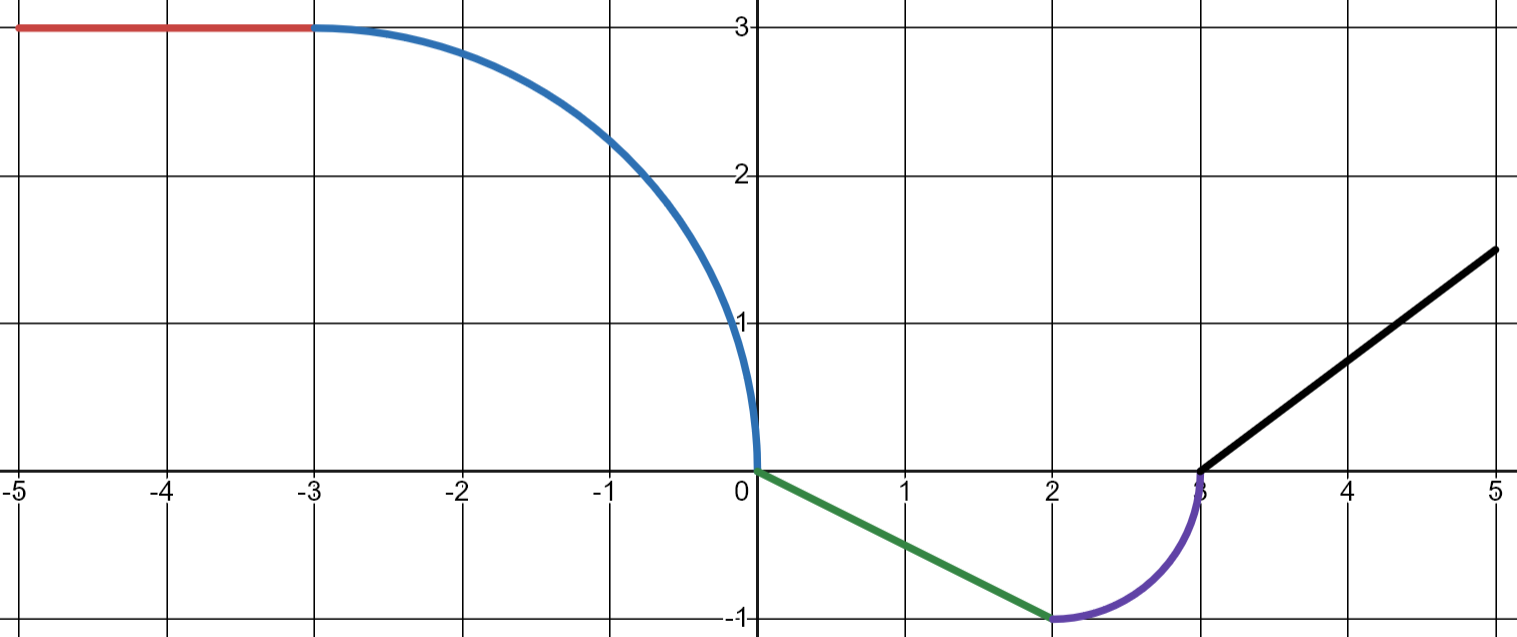
\includegraphics[width=\textwidth]{../images/IN1-v3.png}

Compute each of the following.

\begin{multicols*}{2}
{\everymath{\displaystyle}
\begin{enumerate}[(a)]
    \item $\int_{-5}^{-3} q(t)\ dt$

    \vfill
    \item $\int_{-3}^{0} q(t)\ dt$

    \vfill
    \item $\int_{0}^2 q(t)\ dt$

    \vfill
    \item $\int_2^3 q(t)\ dt$

    \vfill
    \columnbreak
    \item $\int_3^5 q(t)\ dt$

    \vfill
    \item $\int_{-3}^2 q(t)\ dt$

    \vfill
    \item $\int_{-5}^5 q(t)\ dt$

    \vfill
    

\end{enumerate}
}
\end{multicols*}
%%%%%%%%%%%%%%%%%%%%%%%%%%%%%%%%%%%%%%%%%%%%%%%%%%%%%%%%%
\pagebreak

\section{Learning target IN1, version 4}

Use geometric formulas to find definite integrals.

\hrulefill

Here is the graph of a function $N(t)$, which is made up of only straight lines and parts of circles.

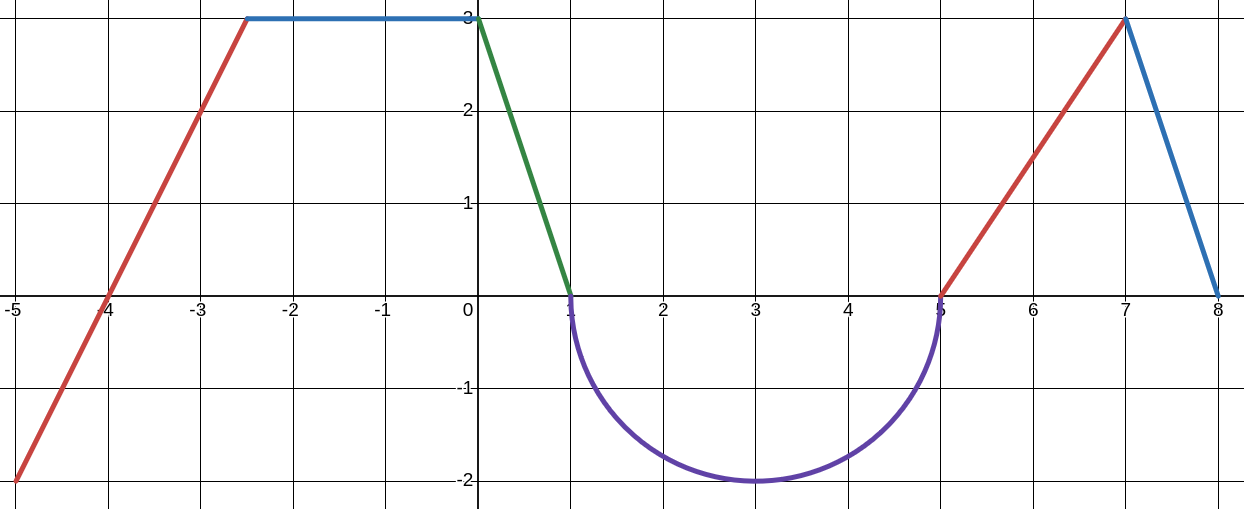
\includegraphics[width=\textwidth]{../images/IN1-v4.png}

Compute each of the following.

\begin{multicols*}{2}
{\everymath{\displaystyle}
\begin{enumerate}[(a)]
    \item $\int_{-5}^{-4} N(t)\ dt$

    \vfill
    \item $\int_{-4}^{-2.5} N(t)\ dt$

    \vfill
    \item $\int_{-2.5}^0 N(t)\ dt$

    \vfill
    \item $\int_0^1 N(t)\ dt$

    \vfill
    \columnbreak
    \item $\int_1^5 N(t)\ dt$

    \vfill
    \item $\int_{5}^7 N(t)\ dt$

    \vfill
    \item $\int_{7}^8 N(t)\ dt$

    \vfill
    \item $\int_{-5}^8 N(t)\ dt$
    

\end{enumerate}
}
\end{multicols*}
%%%%%%%%%%%%%%%%%%%%%%%%%%%%%%%%%%%%%%%%%%%%%%%%%%%%%%%%%
\pagebreak
%%%%%%%%%%%%%%%%%%%%%%%%%%%%%%%%%%%%%%%%%%%%%%%%%%%%%%%%%

\section{Learning target IN2 and INx, version 1}

\iffalse
IN2: Find approximations to definite integrals using variations of Riemann sums.

INx: Correctly interpret the meaning of an area under a curve using the ideas of net change, displacement, etc. Apply the appropriate units to the value.

\hrulefill
\fi

The rate at which pollution escapes a scrubbing process at a manufacturing plant increases over time as filters and other technologies become less effective. Suppose that the rate of pollution (measured in tons per week) is given by the function $r$ that is pictured below. Throughout this problem, we're interested in $\displaystyle\int_{t=0}^5 r(t)\, dt$.

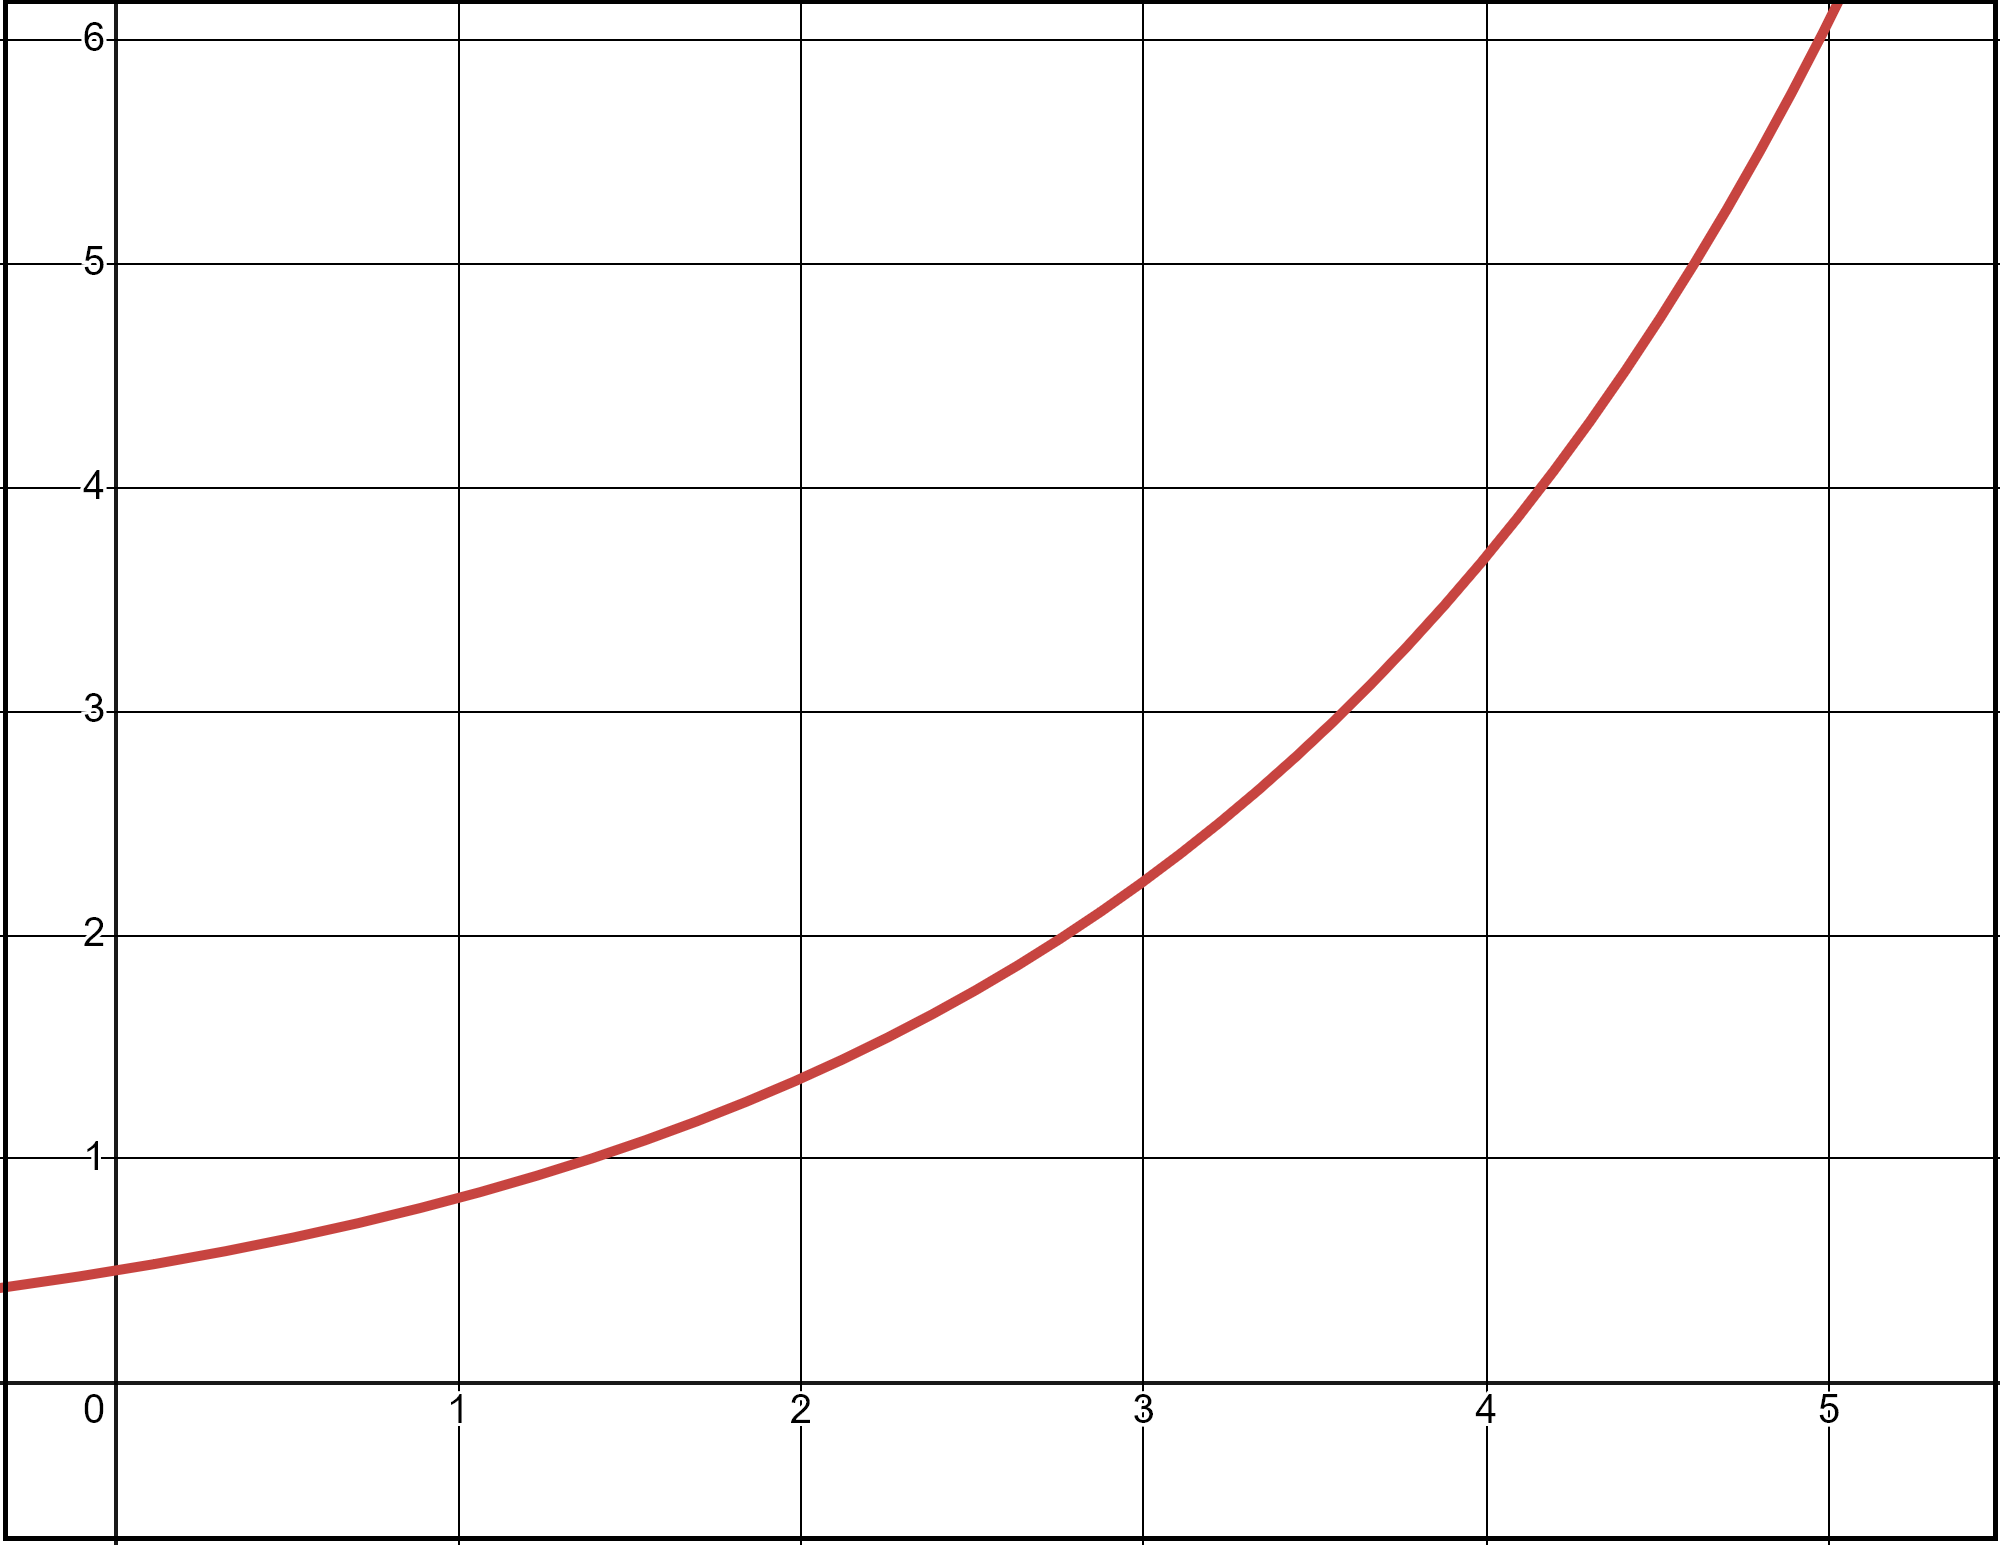
\includegraphics[width=0.5\textwidth]{../images/IN2-v1.png}
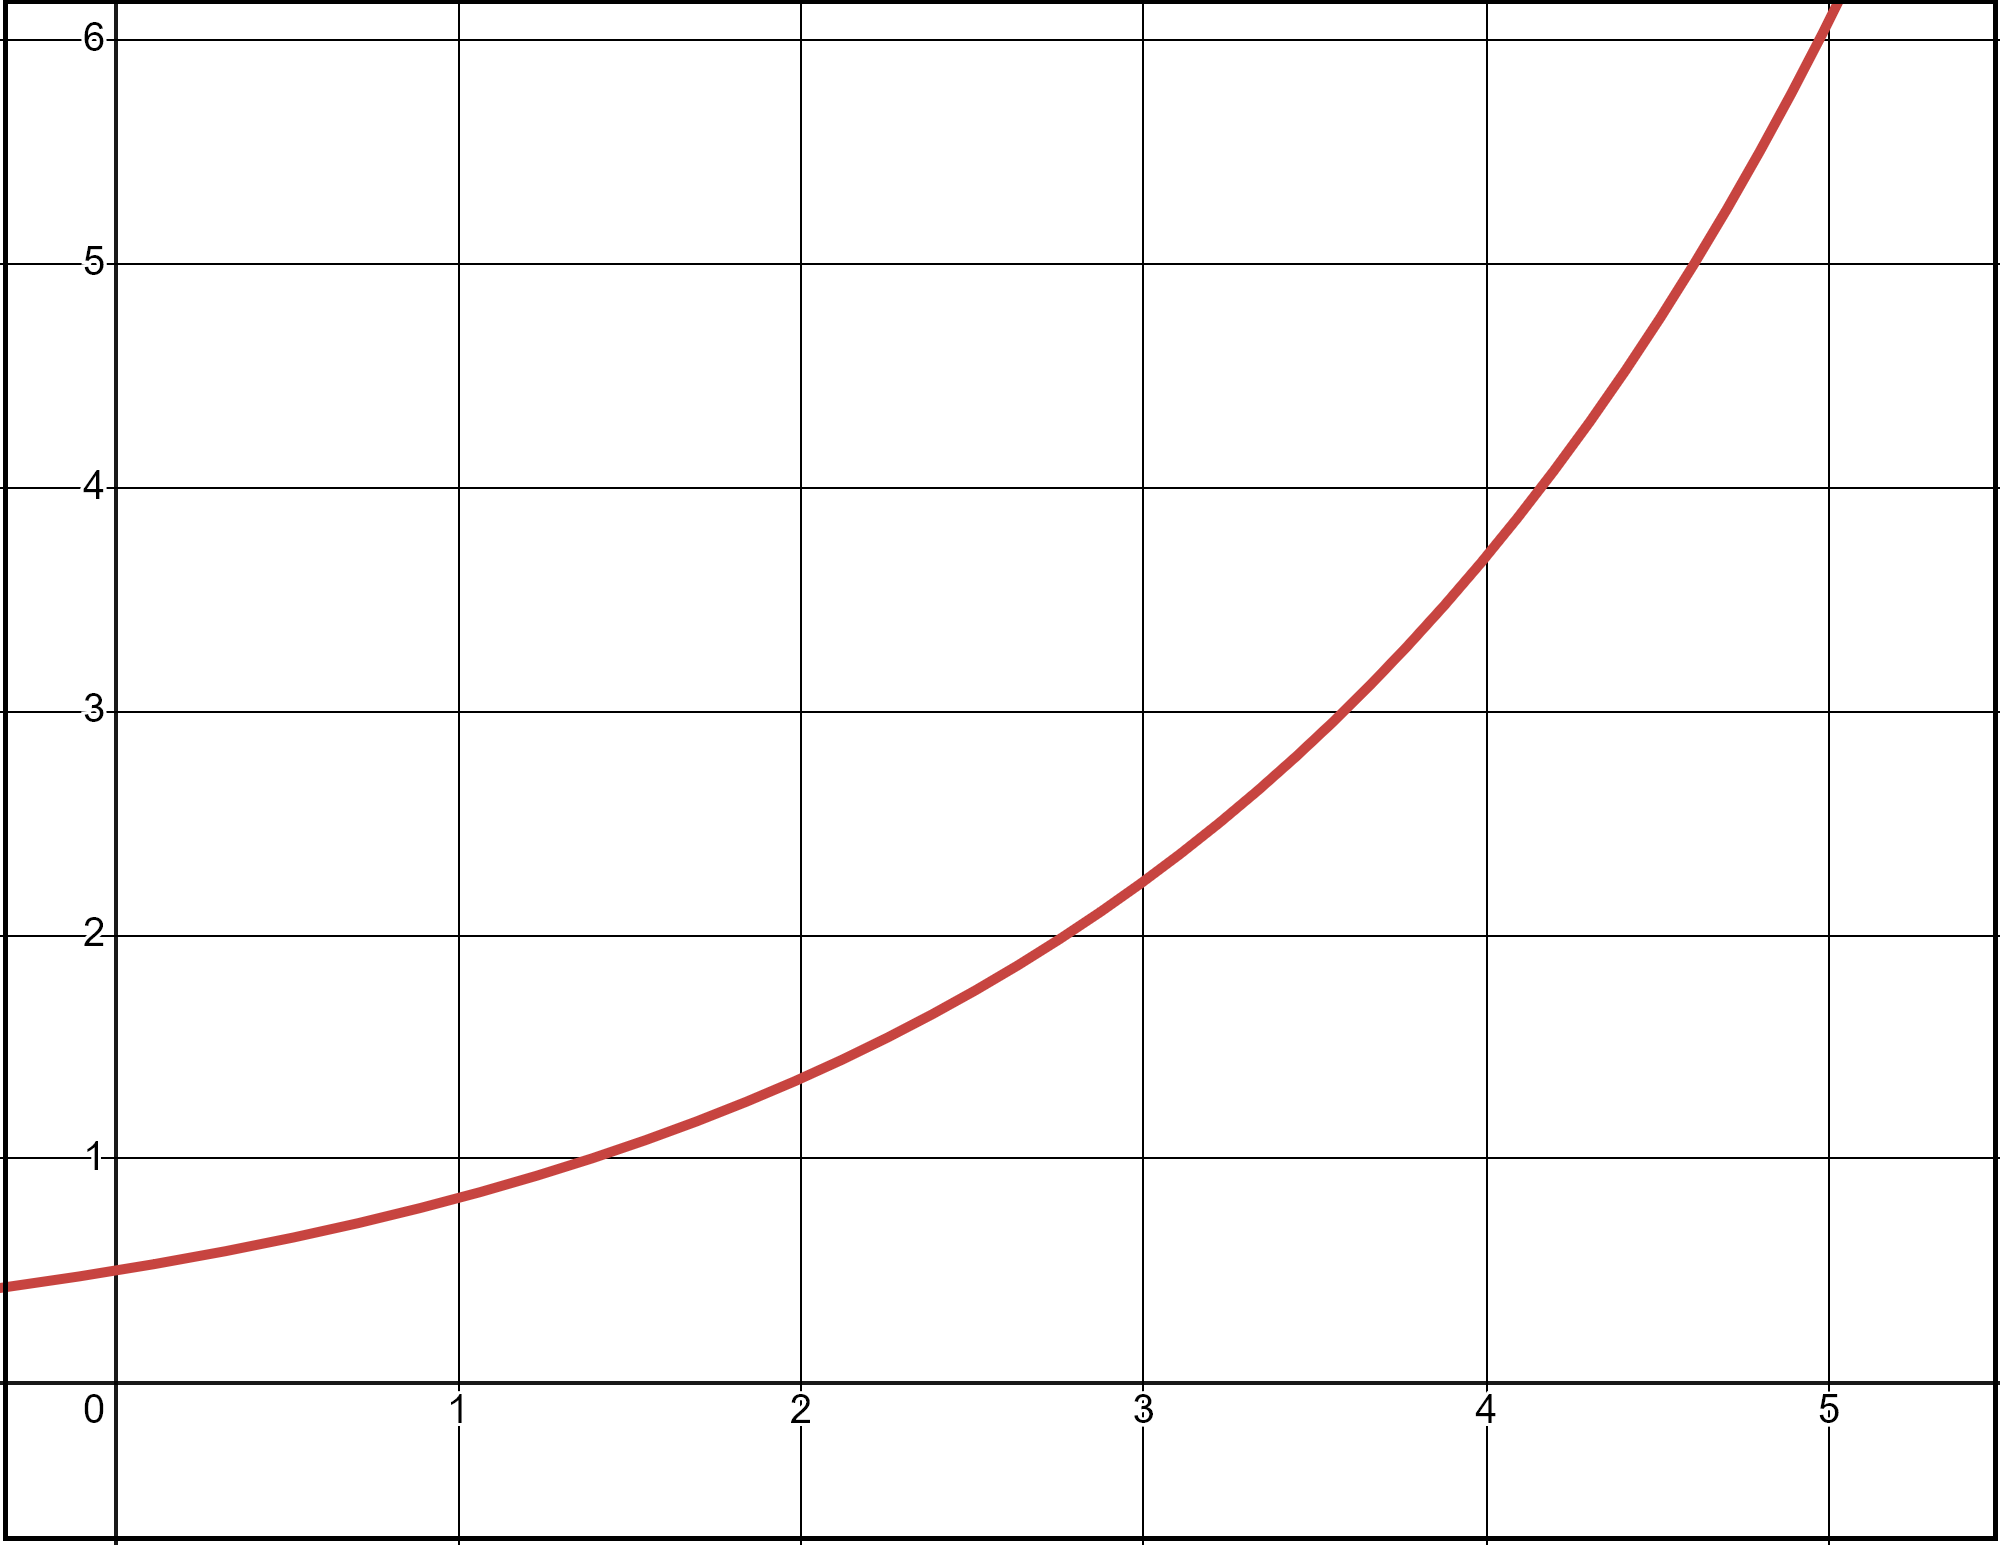
\includegraphics[width=0.5\textwidth]{../images/IN2-v1.png}
\begin{enumerate}[(a)]
\item On the first graph above, carefully draw the \textit{left} Riemann sum with four rectagles of uniform width. (How wide should each rectangle be?)
\item On the second graph above, carefully draw the \textit{right} Riemann sum with four rectangles.
\item If $r(t) = 0.5 e^{0.5t}$, compute both of these Riemann sums. Show your work for computing the heights of the rectangles. (Hint: lots of your work will overlap!)

\textbf{Include units on every number you write.}
\vfill
\item Give your best guess for $\displaystyle\int_{t=0}^5 r(t)\, dt$, \textbf{include units}, and explain what this number means about pollution.
\end{enumerate}
%%%%%%%%%%%%%%%%%%%%%%%%%%%%%%%%%%%%%%%%%%%%%%%%%%%%%%%%%
\pagebreak
%%%%%%%%%%%%%%%%%%%%%%%%%%%%%%%%%%%%%%%%%%%%%%%%%%%%%%%%%

\section{Learning target IN2 and INx, version 2}

\iffalse
IN2: Find approximations to definite integrals using variations of Riemann sums.

INx: Correctly interpret the meaning of an area under a curve using the ideas of net change, displacement, etc. Apply the appropriate units to the value.

\hrulefill
\fi

A colony of bacteria in a petri dish is growing at a rate of 
\(f(t) = 1.75^t\, \text{million bacteria per hour}\). Let's figure out how much the colony grows over the course of three hours.

\fbox{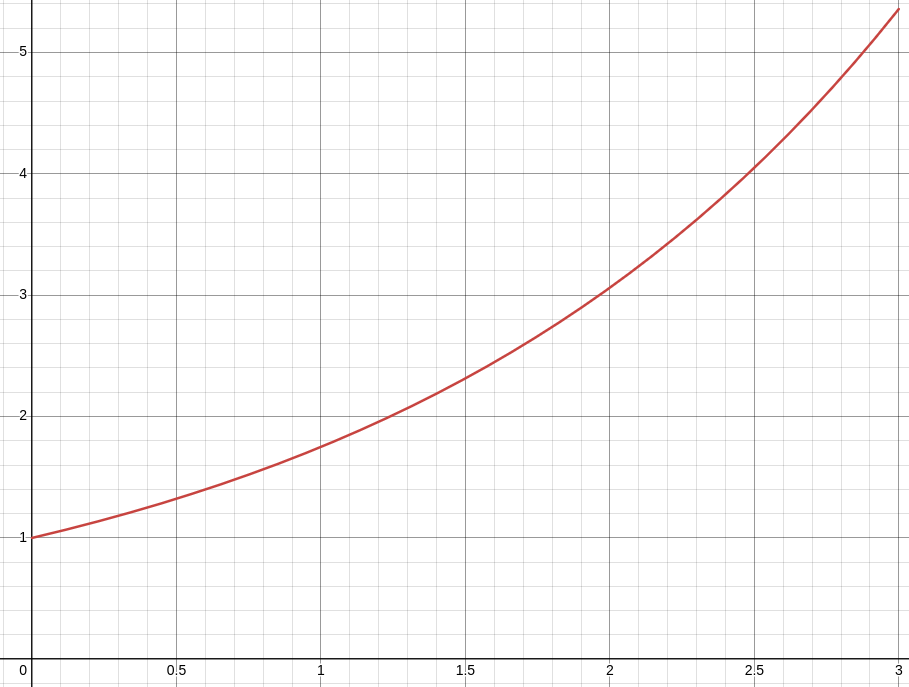
\includegraphics[width=0.5\textwidth]{../images/IN2-v2.png}}
\fbox{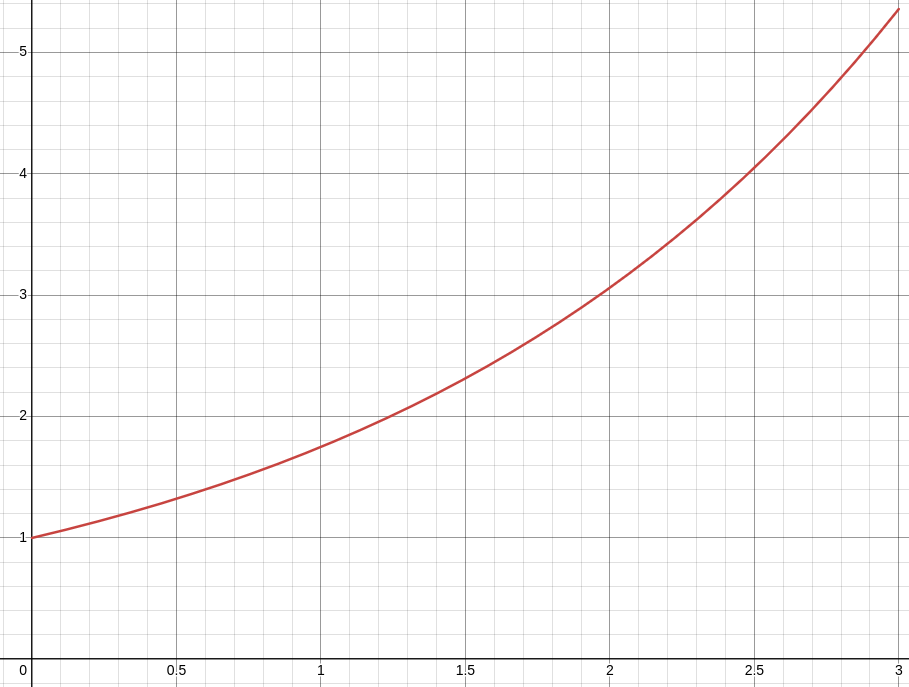
\includegraphics[width=0.5\textwidth]{../images/IN2-v2.png}}
\begin{enumerate}[(a)]
\item On the first graph above, carefully draw the \textit{left} Riemann sum with four rectagles of uniform width. (How wide should each rectangle be?)
\item On the second graph above, carefully draw the \textit{right} Riemann sum with four rectangles.
\item Compute both of these Riemann sums. Show your work for computing the heights of the rectangles. (Hint: lots of your work will overlap!)

\textbf{Include units on every number you write.}
\vfill
\item Give your best guess for $\displaystyle\int_{t=0}^3 f(t)\, dt$, \textbf{include units}, and explain what this number means about the bacteria colony.
\end{enumerate}

%%%%%%%%%%%%%%%%%%%%%%%%%%%%%%%%%%%%%%%%%%%%%%%%%%%%%%%%%
\pagebreak
%%%%%%%%%%%%%%%%%%%%%%%%%%%%%%%%%%%%%%%%%%%%%%%%%%%%%%%%%

\section{Learning target IN2 and INx, version 3}

\iffalse
IN2: Find approximations to definite integrals using variations of Riemann sums.

INx: Correctly interpret the meaning of an area under a curve using the ideas of net change, displacement, etc. Apply the appropriate units to the value.

\hrulefill
\fi

Over the first year of its life, a golden retriever puppy gains weight at a rate of \[p(t) = 4.7 e^{-0.187t} \text{ kilograms per month.}\] 

\fbox{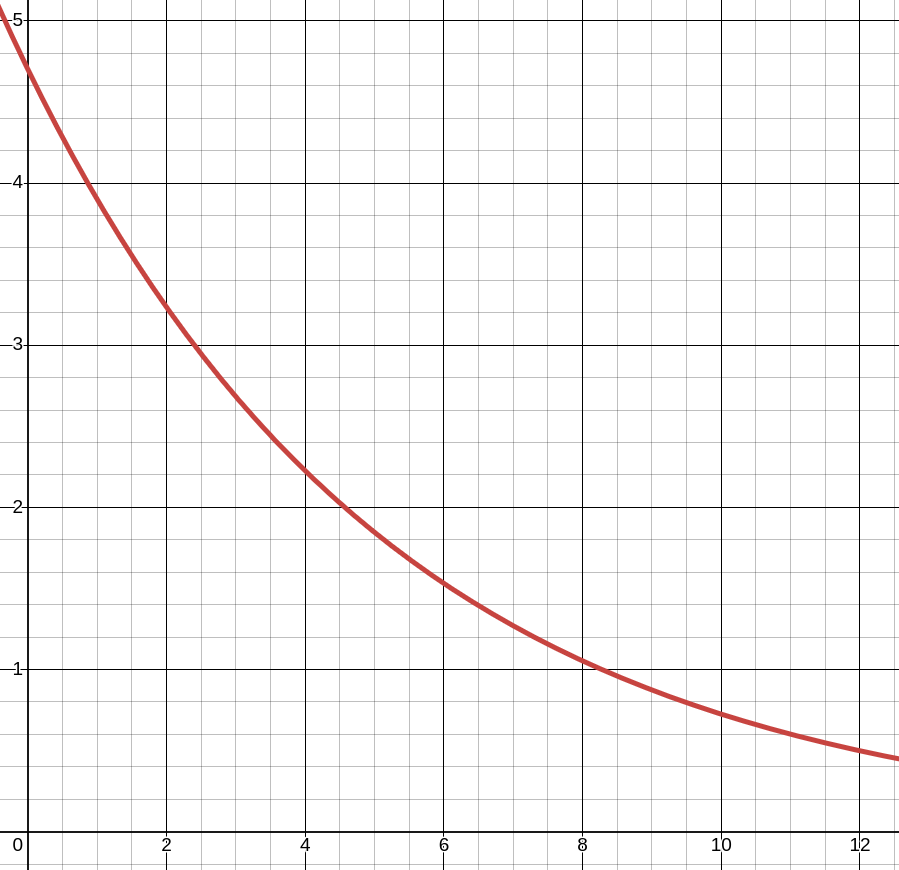
\includegraphics[width=0.5\textwidth]{../images/IN2-v3.png}}
\fbox{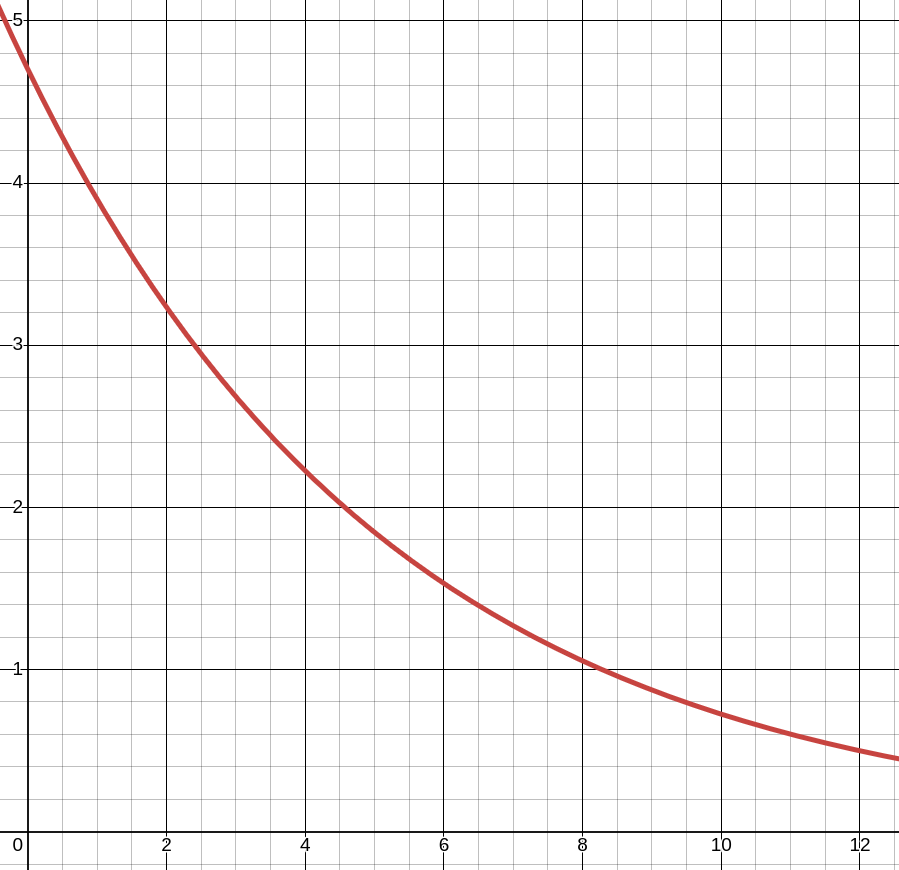
\includegraphics[width=0.5\textwidth]{../images/IN2-v3.png}}
\begin{enumerate}[(a)]
\item On the first graph above, carefully draw the \textit{left} Riemann sum with four rectagles of uniform width. (How wide should each rectangle be?)
\item On the second graph above, carefully draw the \textit{right} Riemann sum with four rectangles.
\item Compute both of these Riemann sums. Show your work for computing the heights of the rectangles. (Hint: lots of your work will overlap!)

\textbf{Include units on every number you write.}
\vfill
\item Give your best guess for $\displaystyle\int_{t=0}^{12} p(t)\, dt$, \textbf{include units}, and explain what this number means about the puppy.
\end{enumerate}

%%%%%%%%%%%%%%%%%%%%%%%%%%%%%%%%%%%%%%%%%%%%%%%%%%%%%%%%%
\pagebreak
%%%%%%%%%%%%%%%%%%%%%%%%%%%%%%%%%%%%%%%%%%%%%%%%%%%%%%%%%

\section{Learning target INx, version 3}

\iffalse
IN2: Find approximations to definite integrals using variations of Riemann sums.

INx: Correctly interpret the meaning of an area under a curve using the ideas of net change, displacement, etc. Apply the appropriate units to the value.

\hrulefill
\fi

Over the first year of its life, a golden retriever puppy gains weight at a rate of \[p(t) = 4.7 e^{-0.187t} \text{ kilograms per month.}\] 
\begin{center}
    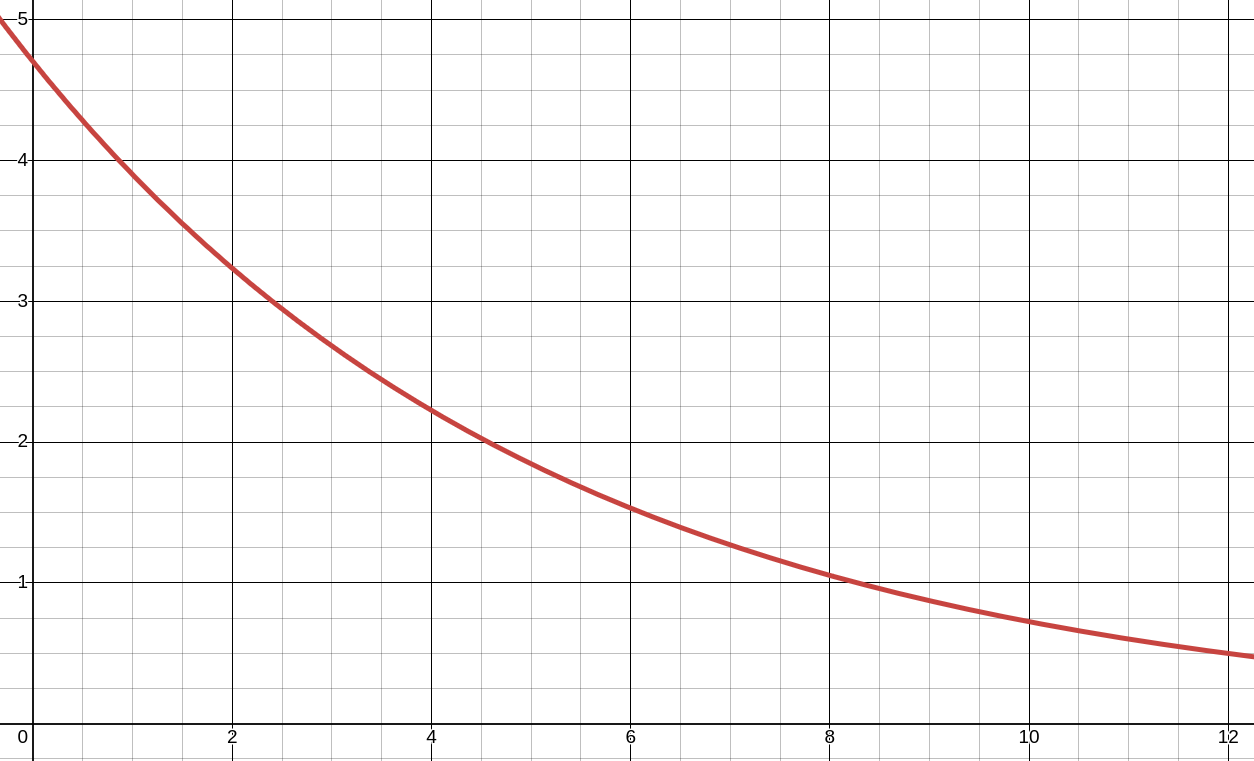
\includegraphics[width=\textwidth]{../images/INx-v3.png}
\end{center}

\begin{enumerate}[(a)]
\item On the graph above, carefully draw a Riemann sum with four rectangles of uniform width. \\(How wide should each rectangle be?)
\item Choose one of the Riemann rectangles you drew and shade it in for clarity. For this rectangle, compute and label:
\vspace{2em}

the height: $\underbrace{\qquad\qquad}_{\text{number}}$ $\underbrace{\quad}_{\text{units}}$
\hfill
the width: $\underbrace{\qquad\qquad}_{\text{number}}$ $\underbrace{\quad}_{\text{units}}$
\hfill
the area: $\underbrace{\qquad\qquad}_{\text{number}}$ $\underbrace{\quad}_{\text{units}}$
\vfill
\item What would the overall area $\displaystyle\int_{t=0}^{12} p(t)\, dt$ mean about the puppy? \textbf{Give units in your answer.}
\end{enumerate}

%%%%%%%%%%%%%%%%%%%%%%%%%%%%%%%%%%%%%%%%%%%%%%%%%%%%%%%%%
\pagebreak
%%%%%%%%%%%%%%%%%%%%%%%%%%%%%%%%%%%%%%%%%%%%%%%%%%%%%%%%%

\section{Learning target INx, version 4}

\iffalse
IN2: Find approximations to definite integrals using variations of Riemann sums.

INx: Correctly interpret the meaning of an area under a curve using the ideas of net change, displacement, etc. Apply the appropriate units to the value.

\hrulefill
\fi

Suppose that an underground storage tank leaks pollutants at a rate of \(r(t)\) gallons per day, where $t$ is measured in days. A researcher studying watershed quality develops the model graphed below:
\[r(t) = 0.0069t^3-0.14t^2+11.485.\]
The researcher is interested in \(\displaystyle\int_{t=2}^{10} r(t)\ dt\).
\begin{center}
    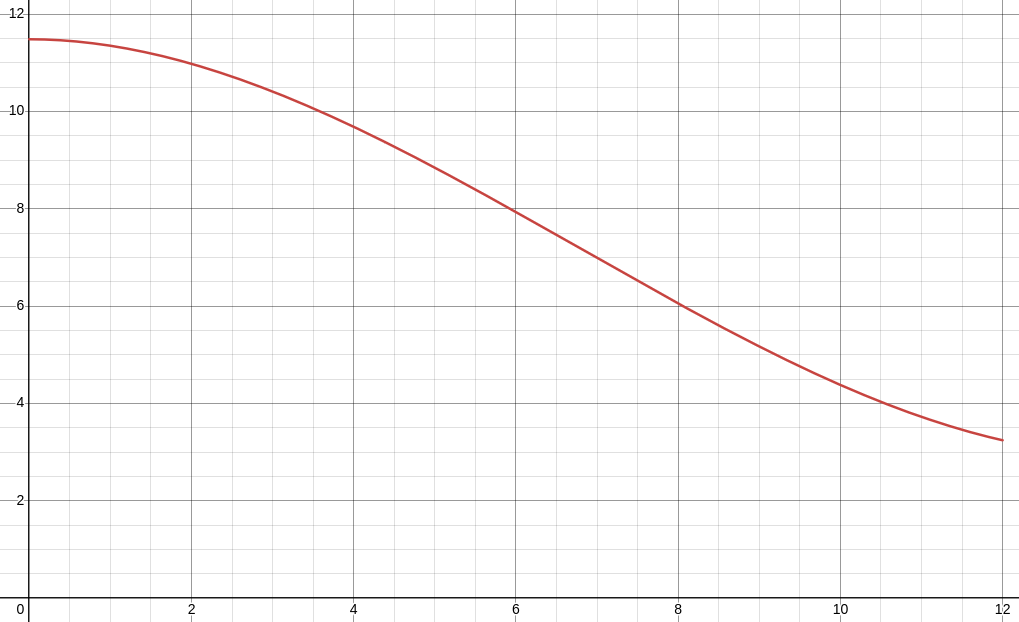
\includegraphics[width=\textwidth]{../images/INx-v4.png}
\end{center}

\begin{enumerate}[(a)]
\item On the graph above, carefully draw a Riemann sum between $t=2$ and $t=10$ with four rectangles of uniform width. \\(How wide should each rectangle be?)
\item Choose one of the Riemann rectangles you drew and shade it in for clarity. For this rectangle, compute and label:
\vspace{2em}

the height: $\underbrace{\qquad\qquad}_{\text{number}}$ $\underbrace{\quad}_{\text{units}}$
\hfill
the width: $\underbrace{\qquad\qquad}_{\text{number}}$ $\underbrace{\quad}_{\text{units}}$
\hfill
the area: $\underbrace{\qquad\qquad}_{\text{number}}$ $\underbrace{\quad}_{\text{units}}$
\vfill
\item What would the overall area $\displaystyle\int_{t=2}^{10} r(t)\, dt$ mean about the watershed? \textbf{Give units!}
\end{enumerate}

%%%%%%%%%%%%%%%%%%%%%%%%%%%%%%%%%%%%%%%%%%%%%%%%%%%%%%%%%
\pagebreak
%%%%%%%%%%%%%%%%%%%%%%%%%%%%%%%%%%%%%%%%%%%%%%%%%%%%%%%%%


\section{Learning target IN3 and IN5, version 1} % checkit 15

Evaluate a definite integral using the Fundamental Theorem of Calculus.

\hrulefill


Explain how to compute the exact value of each of the following definite integrals using the Fundamental Theorem of Calculus. 

\textbf{Leave all answers in exact form, with no decimal approximations. }

\begin{enumerate}[(a)]
\item
 \(\displaystyle \int_{ x=4 }^{ 6 } \left( \frac{6}{x} \right) dx\) 

 \vfill

\item
 \(\int_{x= \frac{5}{4} \, \pi }^{ \frac{4}{3} \, \pi } \left( -2 \, \sec^2\left(x\right) \right) dx\)

\vfill

\item
 \(\int_{x= -2 }^{ -1 } \left( 3 \, x^{3} + 10 \, x - 1 \right) dx\)
\vfill
\end{enumerate}
%%%%%%%%%%%%%%%%%%%%%%%%%%%%%%%%%%%%%%%%%%%%%%%%%%%%%%%%%
\pagebreak

\section{Learning target IN3 and IN5, version 2} 

Evaluate a definite integral using the Fundamental Theorem of Calculus.

\hrulefill


Explain how to compute the exact value of each of the following definite integrals using the Fundamental Theorem of Calculus. 

\textbf{Leave all answers in exact form, with no decimal approximations. }

\begin{enumerate}[(a)]
\item
\(\displaystyle \int_{ x=1 }^{ 5 } \left( \frac{2}{x} + 2^x\right) dx\) 
\vfill
\item 
\(\displaystyle \int_{x=\pi/3}^{3\pi/4} \left( 7\cos(x) \right) dx\)
\vfill
\item
\(\displaystyle \int_{x= -3 }^{ 1 } \left( 9x^3 -9x^2 + 2\right) dx\)
\vfill

\end{enumerate}
%%%%%%%%%%%%%%%%%%%%%%%%%%%%%%%%%%%%%%%%%%%%%%%%%%%%%%%%%
\pagebreak

\section{Learning target IN3 and IN5, version 3} 

Evaluate a definite integral using the Fundamental Theorem of Calculus.

\hrulefill


Explain how to compute the exact value of each of the following definite integrals using the Fundamental Theorem of Calculus. 

\textbf{Leave all answers in exact form, with no decimal approximations. }

\begin{enumerate}[(a)]
\item
\(\displaystyle \int_{x= -2 }^{ 4 } \left( -3x^2 + 4x - 12\right) dx\)
\vfill
\item 
\(\displaystyle \int_{ x=2 }^{ 3 } \left( e^x - \dfrac{3}{x}\right) dx\) 
\vfill
\item
\(\displaystyle \int_{x=\pi/6}^{2\pi/3} \left( 4\sin(x) \right) dx\)
\vfill

\end{enumerate}
%%%%%%%%%%%%%%%%%%%%%%%%%%%%%%%%%%%%%%%%%%%%%%%%%%%%%%%%%
\pagebreak
\section{Learning target IN3 and IN5, version 4} 

Evaluate a definite integral using the Fundamental Theorem of Calculus.

\hrulefill


Explain how to compute the exact value of each of the following definite integrals using the Fundamental Theorem of Calculus. 

\textbf{Leave all answers in exact form, with no decimal approximations. }

\begin{enumerate}[(a)]
\item
\(\displaystyle \int_{x= 0 }^{ \pi } \left( 7\sin(x) - 2x^2\right) dx\)
\vfill
\item 
\(\displaystyle \int_{ x=2 }^{ 10 } \left( \dfrac{3}{x} + 7^x\right) dx\) 
\vfill
\item
\(\displaystyle \int_{x=-1}^{3} \left(9x^4-12x^2+7x-3 \right) dx\)
\vfill

\end{enumerate}
%%%%%%%%%%%%%%%%%%%%%%%%%%%%%%%%%%%%%%%%%%%%%%%%%%%%%%%%%
\pagebreak
%%%%%%%%%%%%%%%%%%%%%%%%%%%%%%%%%%%%%%%%%%%%%%%%%%%%%%%%%

\end{document}